\documentclass{article}
\usepackage[utf8]{inputenc}
\usepackage[margin=0.8in]{geometry}

%\biboptions{sort&compress} %Change citations to be 1-10 if lots are listed

\usepackage{amsmath}
\usepackage{amsfonts} 
\usepackage{amssymb}
\usepackage{bm}
\usepackage{hyperref}

%For tables
\usepackage{booktabs}
\usepackage{multirow}
\usepackage{graphicx}

%For images
\graphicspath{{images/}}

%For subfigures
\usepackage{caption}
\usepackage{subcaption}

%For different coloured text
\usepackage{xcolor}

%For the bibliography
\usepackage[backend=biber,
			  style=ieee,
            sortcites=true,
            sorting=none]{biblatex}

%citestyle=numeric-comp,
%bibstyle=authoryear,       
\addbibresource{Bibliography.bib}

\title{MIL 780 - Assignment Two}
\author{Ryan Balshaw}
\date{05 April 2022}

\begin{document}

\maketitle

\section*{Foreword}
All code, documents and work relevant to this assignment can be found in my \href{https://github.com/RyanBalshaw/MIL_780_assignments}{\textcolor{blue}{Github repository}}.

\section{Question 1}

Consider the following model
\begin{equation}\label{eq:Q1_model}
x_n = \theta  + \epsilon_n,
\end{equation}
where $\epsilon_n \sim \mathcal{N}(0, \sigma^2)$. Given some observed data $\mathbf{x} = [x_1, \cdots, x_N]^T$, the objective is to perform Bayesian inference through a grid-based approach and a conjugate prior approach. The observed data is shown in Figure \ref{fig:Q1_data}.
\begin{figure}[htb!]
\centering
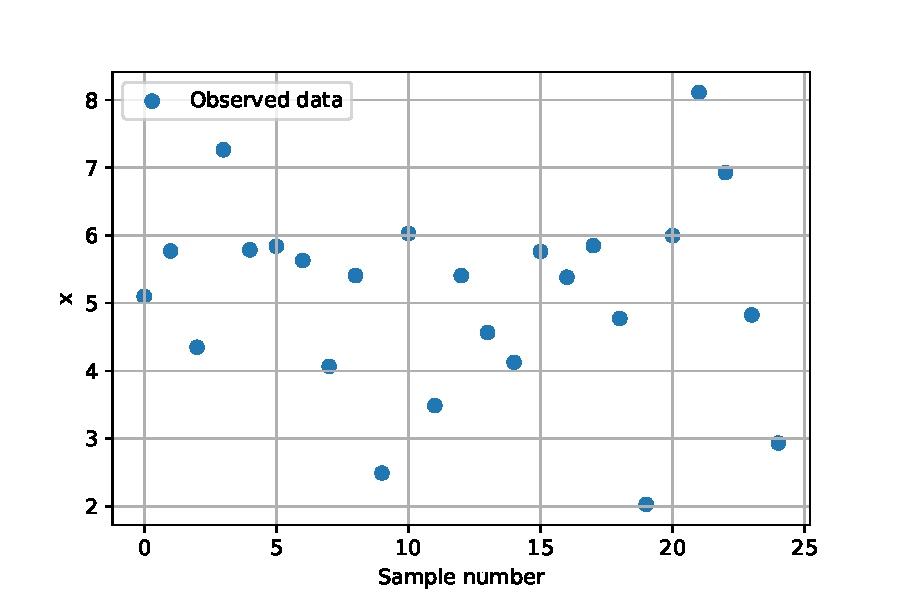
\includegraphics[scale=0.6]{Q1a_1.pdf}
\caption{The observed $x$ data for Question 1.}
\label{fig:Q1_data}
\end{figure}


\subsection{Part A: Grid-based Bayesian inference}

Assume that $\sigma$ is known and given by $\sigma = 1.5$. Assume a Laplacian prior for $\theta$ with the following form:
\begin{equation}
 p(\theta) = L(\theta \vert 0, 2),
\end{equation}    
where 0 is the location parameter and 2 is the scaling parameter. A grid-based approach where $\theta \in [-10, 20]$ is used in the results to follow. There are a number of aspects that are of great important to Bayesian inference:
\begin{itemize}
\item The generative model $p(x \vert \theta)$.
\item The prior $p(\theta)$ over the generative model parameters.
\item The likelihood function $\mathcal{L}(\mathbf{x}, \theta)$.
\item The unnormalised posterior $p(\mathbf{x} \vert \theta)p(\theta)$.
\item The model evidence $p(\mathbf{x})$.
\item The posterior distribution $p(\theta \vert \mathbf{x})$.
\item The posterior predictive distribution $p(x \vert \mathbf{x})$.
\end{itemize}

In this part of the assignment, the objective is to gain exposure to each of these aspects for a simple one-dimensional problem. 

\subsubsection{The prior distribution}
The prior over $\theta$ is given analytically as
\begin{equation}
p(\theta) = L(\mu, b) = \frac{1}{2b} e^{-\frac{\vert x - \mu \vert}{b}},
\end{equation}
and the logarithm of this distribution is equal to
\begin{equation}
\log p(\theta) = -\log ( 2\cdot b ) - \frac{\vert x - \mu \vert}{b}.
\end{equation}
In Figure \ref{fig:Q1a_prior} the prior and the log-prior is shown for $\mu = 0$ and $b = 2$. 
\begin{figure}[htb!]
\centering
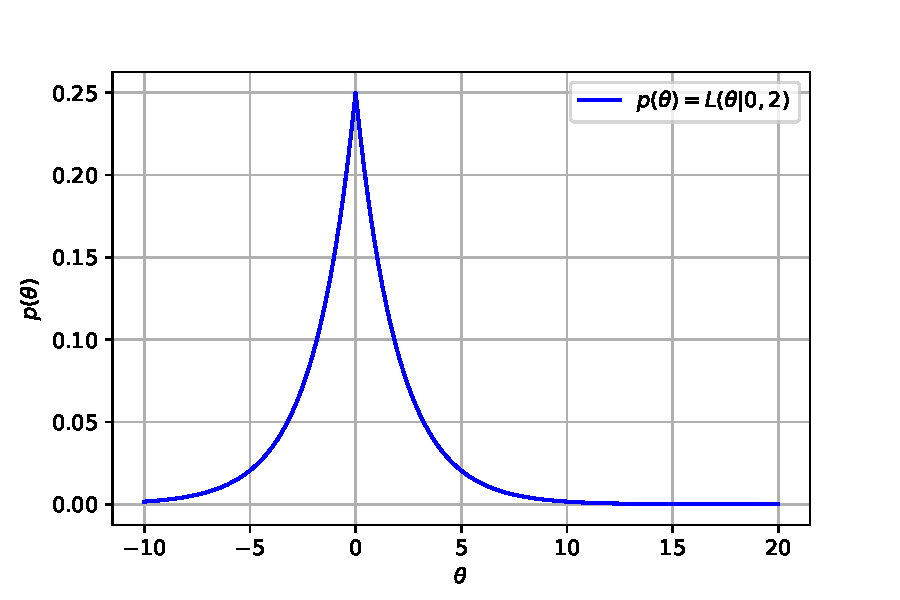
\includegraphics[scale=0.6]{Q1a_2.pdf}
\caption{The prior distribution function $p(\theta)$ visualised over the domain $\theta \in [-10, 20]$.}
\label{fig:Q1a_prior}
\end{figure}


\subsubsection{The generative model and the likelihood function}

Given the model in Equation \eqref{eq:Q1_model}, the model distribution over x is given as
\begin{equation}
\begin{aligned}[b]
p(x \vert \theta) &= \mathcal{N}(x \vert \theta, \sigma^2) \\
&= \frac{1}{\sqrt{2 \cdot \pi \cdot \sigma^2}} e^{-\frac{1}{2\sigma^2} \cdot \left( x - \theta \right)^2}.
\end{aligned}
\end{equation}
Given some observed data $\mathbf{x}$, where $\mathbf{x}$ is a column vector $\mathbf{x} \in \mathbb{R}^{N \times 1}$ and $N$ is the number of observed samples, the likelihood function, given $\theta$, is
\begin{equation}
\mathcal{L}(\mathbf{x}, \theta) = \prod_{n=1}^{N} p(x_n \vert \theta).
\end{equation}
The log-likelihood function may be given as
\begin{equation}
\begin{aligned}[b]
\mathcal{LL}(\mathbf{x}, \theta) &= \sum_{n=1}^{N} \log p(x_n \vert \theta) \\
&= \sum_{n=1}^{N} \left[ -\frac{1}{2}\log (2\cdot \pi) - \frac{1}{2}\log (\sigma^2) - \frac{\left( x - \theta \right)^2}{2\sigma^2} \right] \\
&= -\frac{N}{2}\log (2\cdot \pi) - \frac{N}{2}\log (\sigma^2) - \sum_{n=1}^{N} \left[\frac{\left( x - \theta \right)^2}{2\sigma^2} \right].
\end{aligned}
\end{equation}
It is important here to remind ourselves (read: myself) of the functions of the $\mathcal{LL}$ function. The observed data is typically fixed, and thus the only variable that we can alter is $\theta$. Thus, we can plot how the likelihood/log-likelihood function varies with $\theta$. In Figure \ref{fig:Q1a_likelihood} the likelihood function and log-likelihood function over $\theta$ is shown. Furthermore, the likelihood function is the joint probability of the observed data given the model parameters. In Bayesian inference, the likelihood function is key to finding the posterior distribution $p(\theta \vert \mathbf{x})$.
\begin{figure}[htb!]
\centering
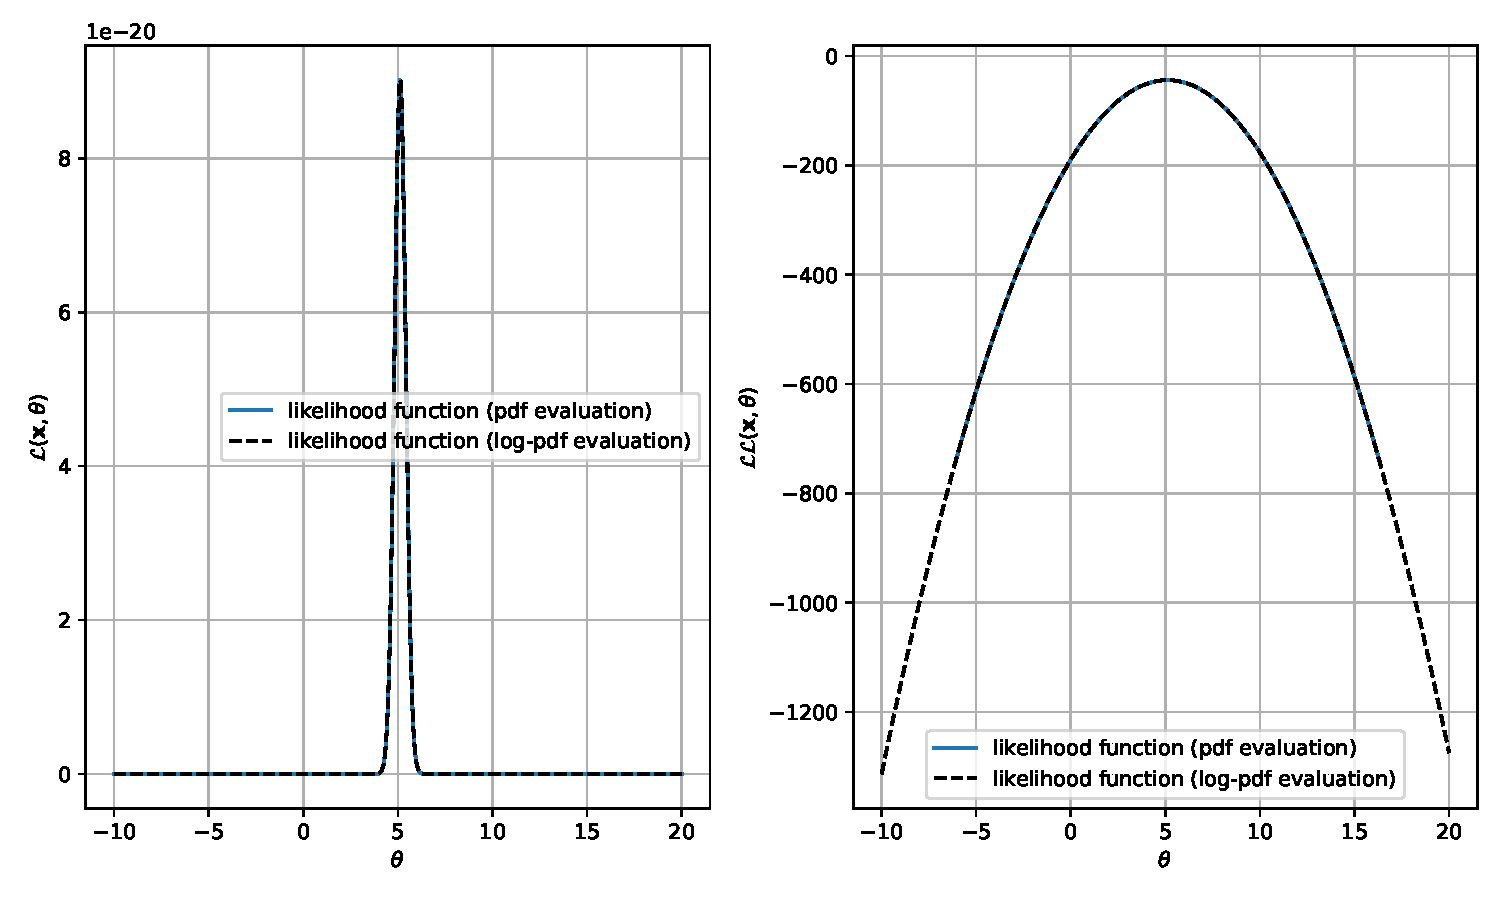
\includegraphics[scale=0.6]{Q1a_3.pdf}
\caption{The likelihood function $\mathcal{L}(\mathbf{x}, \theta)$ of the generative model $p(x \vert \theta)$ over the domain $\theta \in [-10, 20]$. In a) the likelihood function is shown, and in b) the log-likelihood function is shown.}
\label{fig:Q1a_likelihood}
\end{figure}

\subsubsection{The unnormalised posterior}
The unnormalised posterior is the numerator of posterior distribution over $\theta$ given $\mathbf{x}$. The posterior is given through Bayes' rule
\begin{equation}\label{eq:Q1_Bayes}
p(\theta \vert \mathbf{x}) = \frac{p(\mathbf{x}\vert\theta)p(\theta)}{p(\mathbf{x})}.
\end{equation}
It is now clear why the prior was the first step of the Bayesian process. We assume a prior over $\theta$, observe some data $\mathbf{x}$ and then we can inspect the posterior $p(\theta \vert \mathbf{x})$. To do this, we need the unnormalised posterior $p(\mathbf{x}\vert\theta)p(\theta)$ and the model evidence $p(\mathbf{x})$. To determine the unnormalised posterior we can use the analytical forms of the likelihood function and the prior distribution
\begin{equation}
\begin{aligned}[b]
p(\mathbf{x}, \theta) &= p(\mathbf{x}\vert\theta)p(\theta) \\
\mathcal{F}(\theta, \mathbf{x}, , \sigma, \mu_\theta, b) &= \frac{1}{2 \cdot b} \exp{ \left(- \frac{\vert \theta - \mu_\theta \vert}{b} \right)} \prod_{n=1}^{N} \frac{1}{ \sqrt{2 \cdot \pi \cdot \sigma^2}} \exp{ \left(-\frac{1}{2\sigma^2} \cdot \left( x_n - \theta \right)^2 \right)},
\end{aligned}
\end{equation}
where $\mathcal{F}(\theta, \mathbf{x}, \sigma, \mu_\theta, b)$ is the notation that I have adopted to show the parameters of the unnormalised posterior. In this case, $\sigma$, $\mu_\theta$ an $b$ are fixed to $\sigma =1.5$,  $\mu_\theta = 0$ and $b = 2$. It is also possible to inspect the log-unnormalised posterior, and this is given analytically as
\begin{equation}
\begin{aligned}[b]
\log p(\mathbf{x}, \theta) &= \log p(\mathbf{x}\vert\theta) + \log p(\theta) \\
\mathcal{LF}(\theta, \mathbf{x}, , \sigma, \mu_\theta, b) &= \sum_{n=1}^{N} \left[ -\frac{1}{2}\cdot\log (2\cdot \pi) - \frac{1}{2}\cdot\log (\sigma^2) - \frac{\left( x_n - \theta \right)^2}{2\sigma^2} \right]  -\log ( 2\cdot b ) - \frac{\vert \theta - \mu_\theta \vert}{b} \\ 
&= -\frac{N}{2} \cdot \log (2\cdot \pi) - \frac{N}{2} \cdot \log (\sigma^2) - \log ( 2\cdot b ) - \frac{\vert \theta - \mu_\theta \vert}{b} - \sum_{n=1}^{N} \frac{\left( x_n - \theta \right)^2}{2\sigma^2}.
\end{aligned}
\end{equation}
In Figure \ref{fig:Q1a_unnorm_posterior} the unnormalised posterior is shown. Notice how the prior and likelihood function influences the unnormalised posterior. There appears to be a slight shift towards the origin, and the influence of the prior is marginal in comparison to the likelihood function. The marginal influence of the prior is attributed to the prior parameters, as the prior is far from the likelihood function and the variance ensures that the prior is numerically larger over the $\theta$ domain in comparison to the likelihood function. Decreasing the variance or shifting the prior mean should increase its influence on the unnormalised posterior.  
\begin{figure}[htb!]
\centering
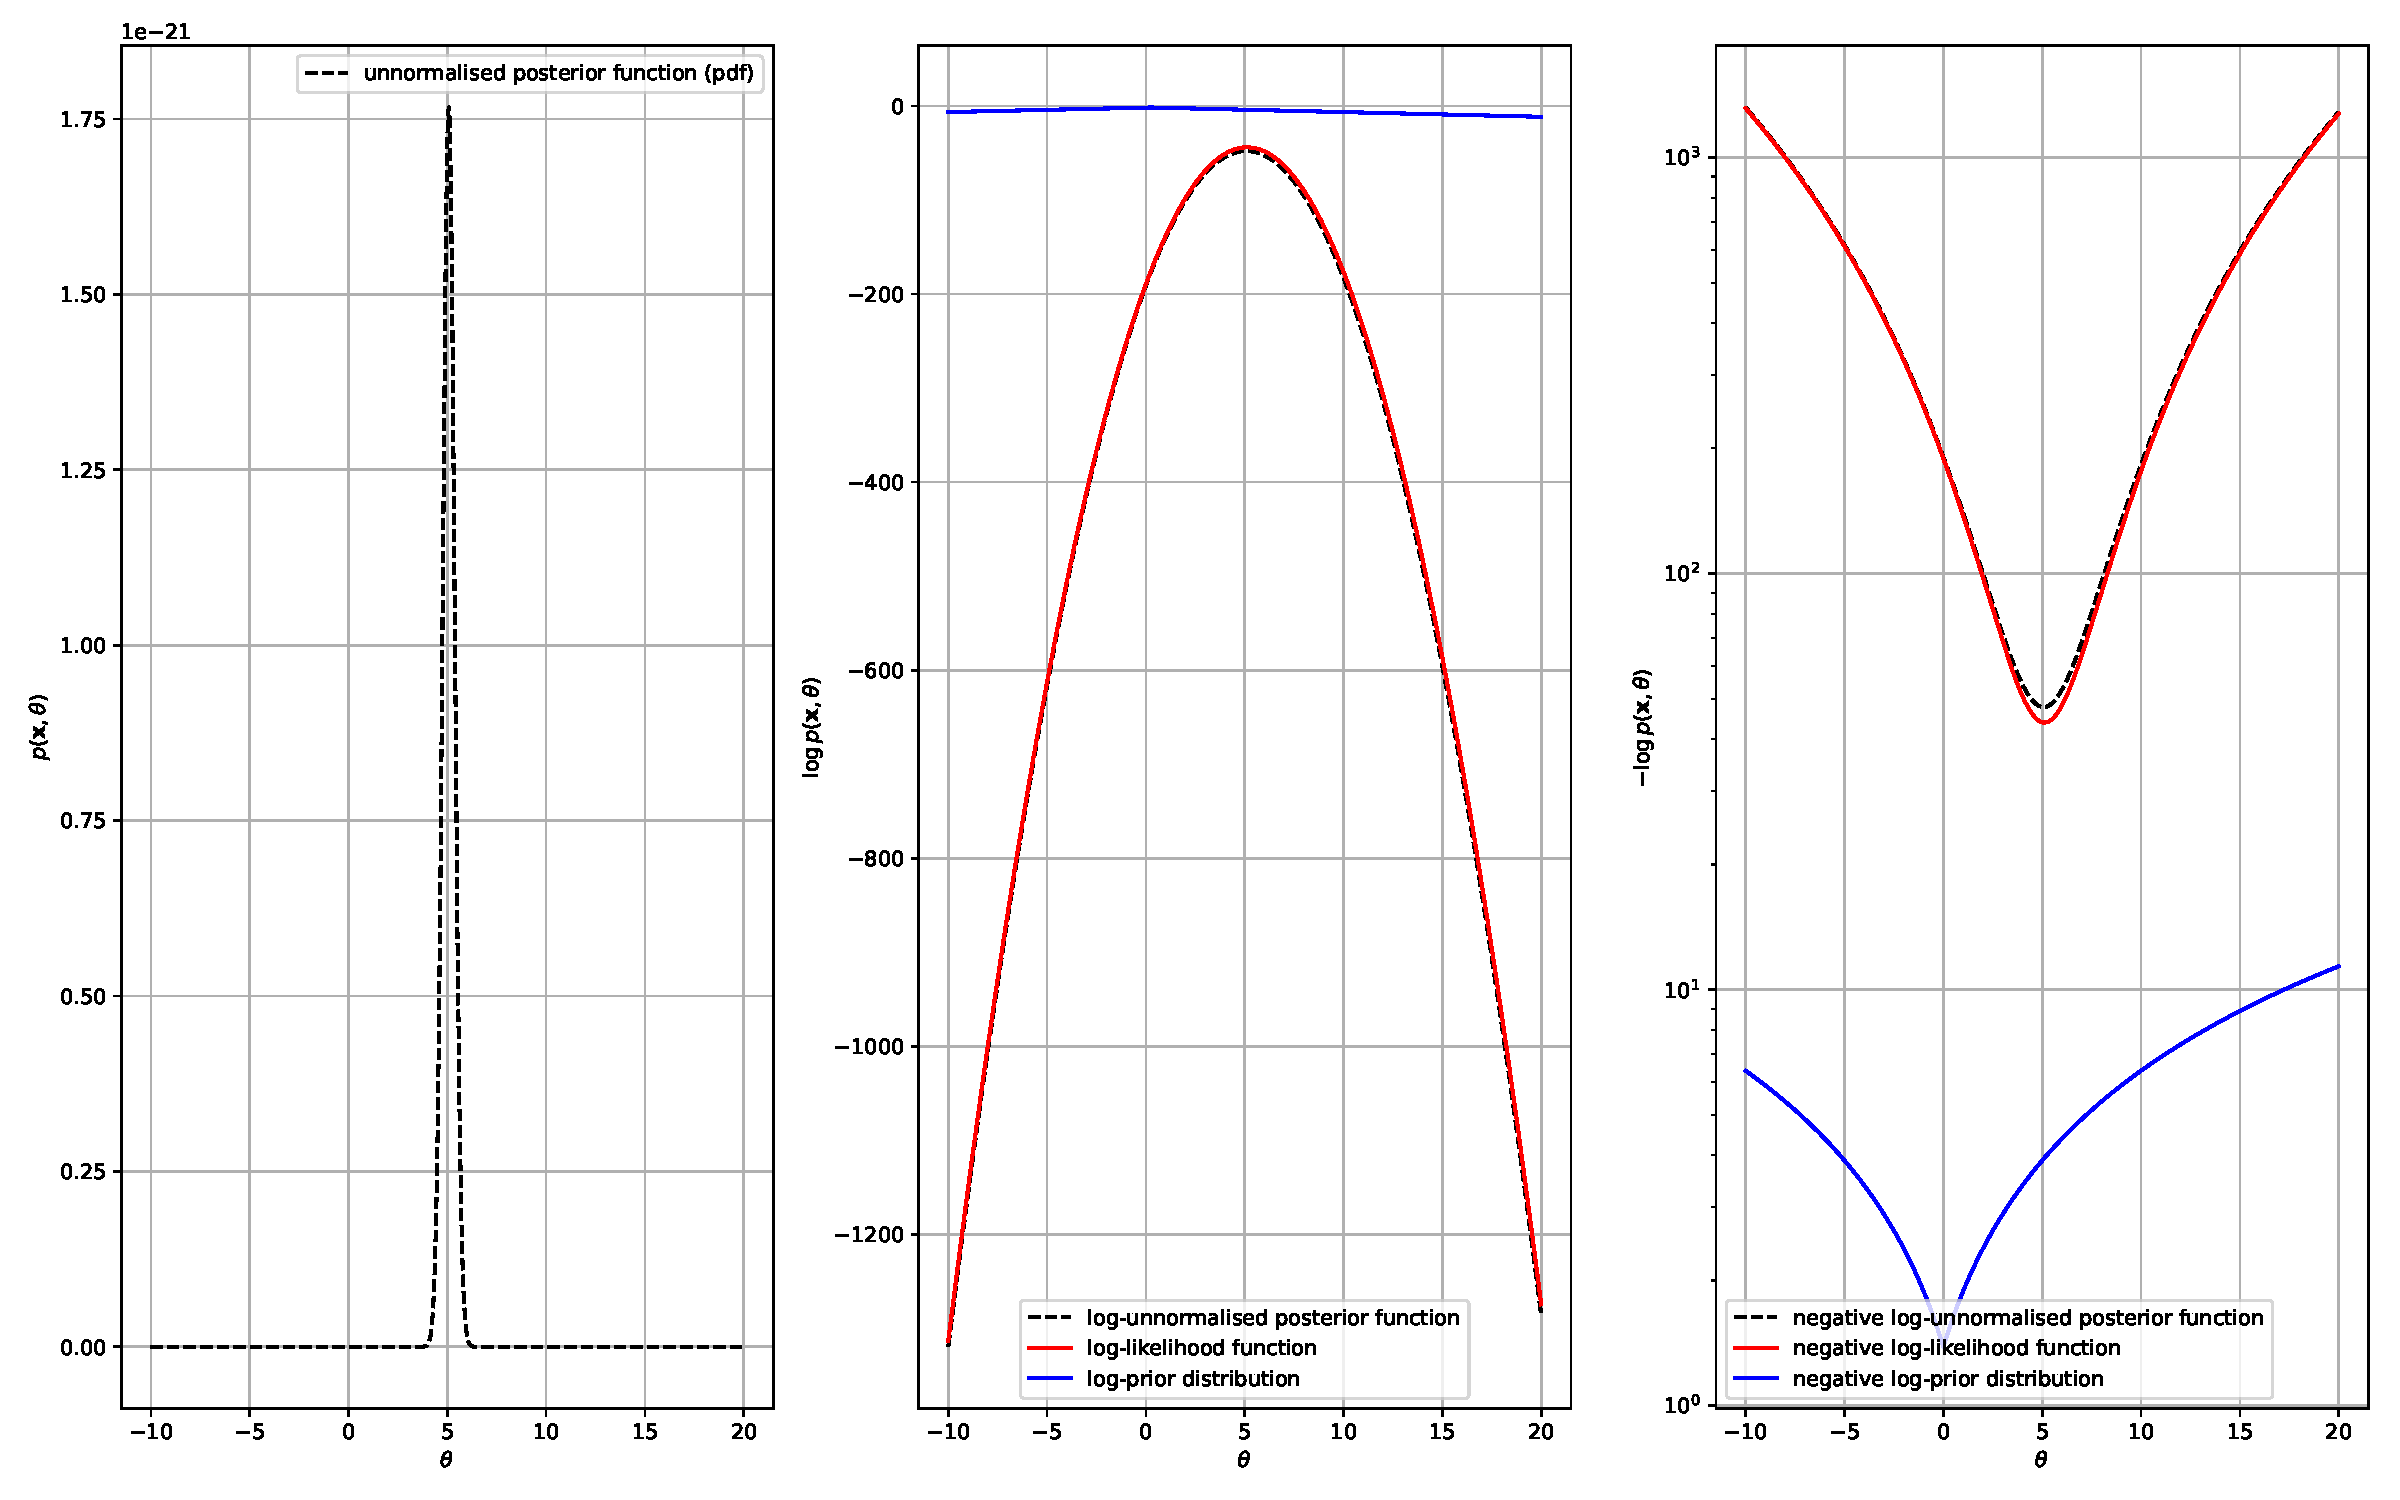
\includegraphics[scale=0.4]{Q1a_4.pdf}
\caption{The unnormalised posterior distribution $\mathcal{F}(\theta, \mathbf{x}, \sigma, \mu_\theta, b)$ for $\sigma  =1.5, \mu_\theta = 0$ and $b = 2$ over the domain $\theta \in [-10, 20]$. Three variations of the unnormalised posterior is visualised here, the standard unnormalised posterior, the logarithm of the unnormalised posterior and the terms therein, and the negative of the unnormalised log-posterior.}
\label{fig:Q1a_unnorm_posterior}
\end{figure}

\subsubsection{The model evidence}
In order to determine the posterior distribution over the parameters $p(\theta \vert \mathbf{x})$, we need to determine the denominator of Equation \eqref{eq:Q1_Bayes}. The denominator is commonly referred to as the model evidence, and it is sometimes known as the marginal likelihood $p(\mathbf{x})$. Note that this marginalisation is with respect to the generative model parameters and represents the probability of the observed data marginalized over the parameters $\theta$. This is given formally as
\begin{equation}
\begin{aligned}[b]
p(\mathbf{x}) &= \int_\theta p(\mathbf{x}, \theta) d\theta \\
&= \int_\theta p(\mathbf{x} \vert \theta) p(\theta) d\theta \\
&= 1.32856e^{-21}.
\end{aligned}
\end{equation}

\subsubsection{The posterior distribution}
Now that we know the model evidence, we can use the unnormalised posterior and normalise it by the model evidence to obain the posterior distribution $p(\theta \vert \mathbf{x})$. In Figure \ref{fig:Q1a_posterior} the posterior distribution for the model parameter $\theta$ is shown. Notice how the model evidence, which is a constant, effectively rescales the unnormalised posterior. This is to ensure that the posterior distribution is a true distribution (i.e., it satisfies $\int_\theta p(\theta \vert \mathbf{x})d\theta = 1$ and $p(\theta \vert \mathbf{x}) > 0$  $\forall$  $\theta$).
\begin{figure}[htb!]
\centering
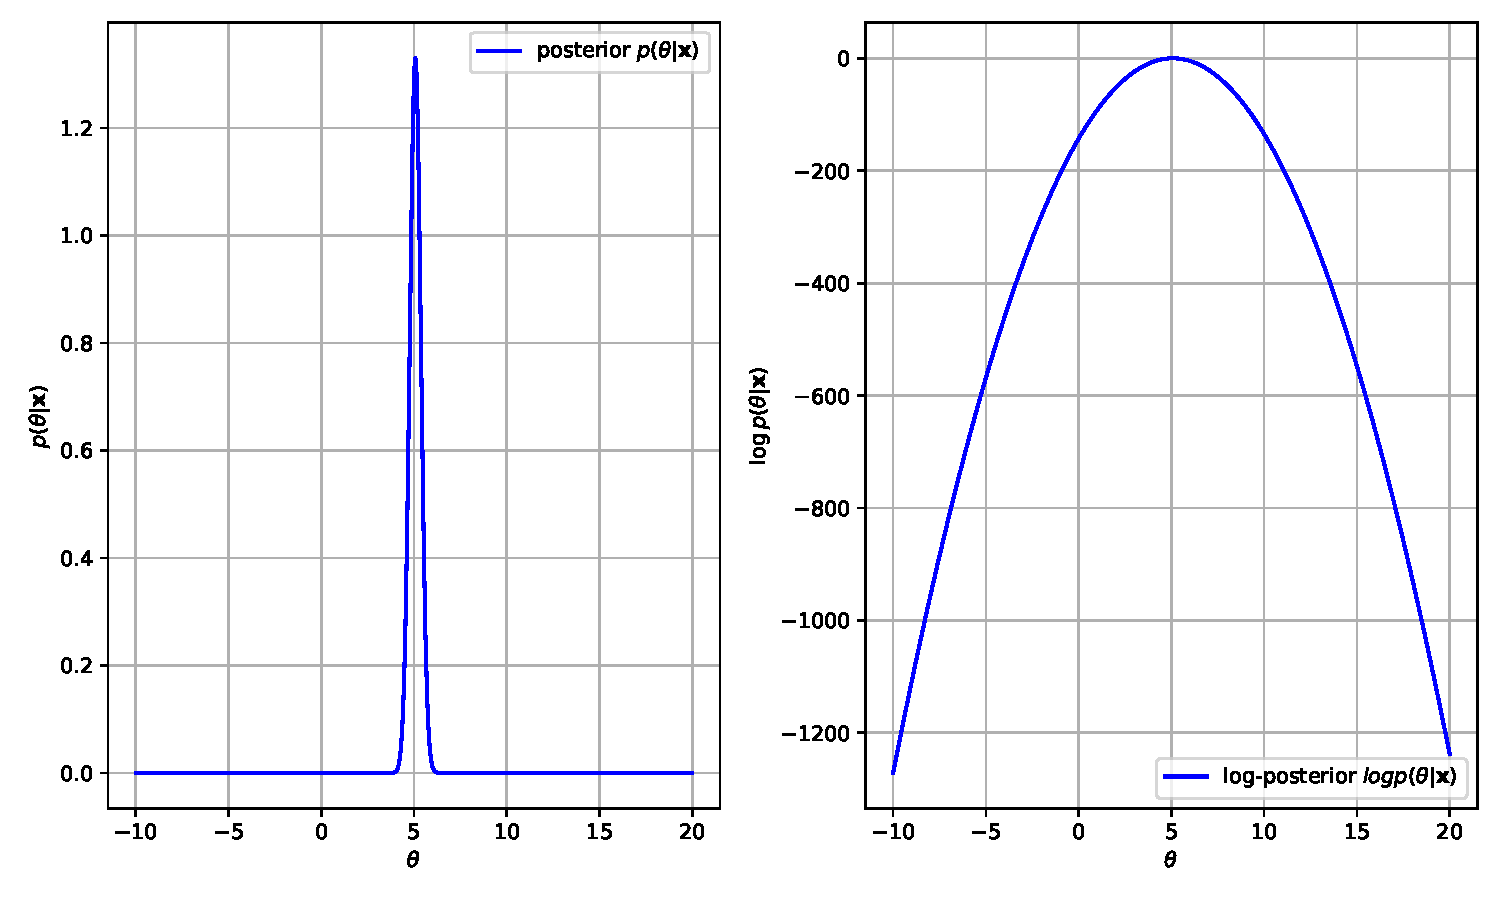
\includegraphics[scale=0.6]{Q1a_5.pdf}
\caption{The posterior distribution $p(\theta \vert \mathbf{x})$ and the logarithm thereof over the domain $\theta \in [-10, 20]$. The MAP solution is given in Table \ref{tab:Q1_a}.}
\label{fig:Q1a_posterior}
\end{figure}

\subsubsection{The posterior predictive distribution}
However, finding the posterior distribution is only only part of the Bayesian inference puzzle. We would still like to use the generative model given in Equation \eqref{eq:Q1_model} for any newly observed data and to do so, we need to incorporate the posterior distribution in some way. A naive, but viable approach is to use the maximum-a-posteriori (MAP) estimate from the unnormalised posterior as a basis for the model parameter $\theta$. However, this is simply a parameter re-substitution of the estimator for $\theta$ and is equivalent to maximum likelihood estimation. The power of Bayesian inference is that we can incorporate all uncertainty in the unknown parameter when observing new data. This allows us to quantify new data under all possible variations of the unknown model parameter $\theta$ rather than on a maximum estimate\footnote{I found the following \href{https://stats.stackexchange.com/questions/242082/posterior-predictive-distribution-vs-map-estimate}{\textcolor{blue}{StackExchange}} discussion very insightful.}. To use the uncertainty of the unknown parameter for newly observed data, we can use the posterior predictive distribution. This is given as 
\begin{equation}\label{eq:Q1a_posterior}
p(x\vert \mathbf{x}) = \int_\theta p(x \vert \theta) p(\theta \vert \mathbf{x}) d\theta.
\end{equation}
In Figure \ref{fig:Q1a_posterior_predictive} the posterior predictive distribution is shown. In my implementation I used two methods to numerically estimate the integral in Equation \eqref{eq:Q1a_posterior}. The expensive version, where I used \texttt{scipy.integrate.quad}, took 202.154 seconds to perform 1000 iterations over $x$. The cheap version, where I used \texttt{scipy.integrate.trapz}, took 0.039 seconds to perform 1000 iterations over $x$. 
\begin{figure}[htb!]
\centering
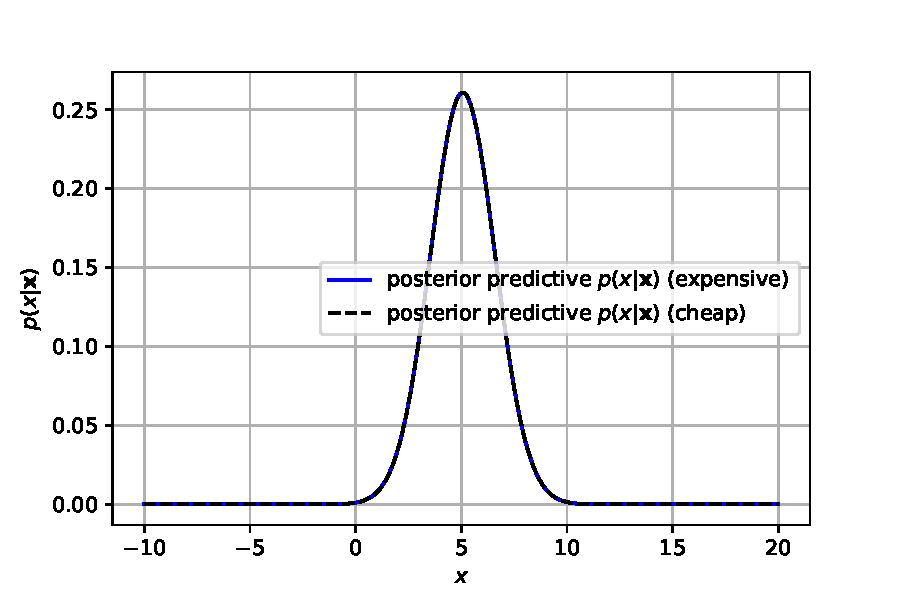
\includegraphics[scale=0.6]{Q1a_6.pdf}
\caption{The posterior predictive distribution $p(x \vert \mathbf{x})$ determined using a cheap and expensive computational methodology over the domain $\theta \in [-10, 20]$.}
\label{fig:Q1a_posterior_predictive}
\end{figure}

\subsubsection{Estimating estimators}
We can now compare different estimators for the unknown parameter $\theta$ using the prior distribution, the likelihood function and the unnormalised posterior function. This estimator estimation process can be performed using a grid-based approach, analytical solutions and through numerical optimisation techniques. In Table \ref{tab:Q1_a} the estimates for these three approaches is given. Notice how the MAP estimate is lower than the maximum likelihood (ML) estimate, which is due to the influence of the prior $p(\theta)$.
\begin{table}[htb!]
\centering
\caption{The estimates for the unknown parameter $\theta$ using the prior, maximum likelihood and maximum a posteriori. These estimates are found using a grid-based approach, analytically and through numerical optimisation.}
\label{tab:Q1_a}
\begin{tabular}{@{}cccc@{}}
\toprule
Approach & Prior & ML & MAP \\ \midrule
Grid-based & 0.0 & 5.1051 & 5.075 \\
Analytical & -0.0002 & 5.1161 & N/A \\
Numerical & 0.002737 & 5.1161 & 5.071 \\ \bottomrule
\end{tabular}
\end{table}

\subsubsection{Using Bayesian inference}
We can use the posterior distribution $p(\theta \vert \mathbf{x})$ and the posterior predictive distribution $p(x \vert \mathbf{x})$ to determine probabilities $p(a \leq X \leq b)$. The first probability of interest is $p(\theta \leq 4 \vert \mathbf{x})$ and the second is $p(x \leq 4 \vert \mathbf{x})$. As a reminder, the probability $p(a \leq x \leq b)$ may be given as
\begin{equation}
p(a \leq x \leq b) = F_x(b) - F_x(a),
\end{equation}
where $F_x(X) = \int_{-\infty}^{X} p(x) dx$ is the cumulative distribution function (CDF) of $p(x)$. As we do not know the analytical forms of the posterior and posterior predictive distributions, we cannot use an analytical expression for the CDFs. However, we have a discretised set of likelihoods along the $\theta$ and $x$ domain and thus we can estimate the CDF by cumulatively adding the likelihoods. It is assumed here that the CDF varies linearly between points along each respective domains. A linear interpolation approach is then used to estimate $F_x(X)$. This process ensures that we can estimate the probabilities of interest.

Using this approach, it was found that $p(\theta \leq 4 \vert \mathbf{x}) = 0.0002$ and $p(x \leq 4 \vert \mathbf{x}) = 0.2419$. In Figure \ref{fig:Q1a_CDFs} the CDFs of interest and the resulting probabilities are shown. The posterior probability that $\theta \leq 4$ informs us that it is very unlikely that a model parameter $\theta$ in this range is responsible for generating the observed data. The posterior predictive probability that $x \leq 4$ is noticeably larger, and this indicates that it is far more probable that newly observed $x$ samples may be drawn in the $x$ domain $x \in [-\infty, 4]$. 
\begin{figure}
     \centering
     \begin{subfigure}[b]{0.45\textwidth}
         \centering
         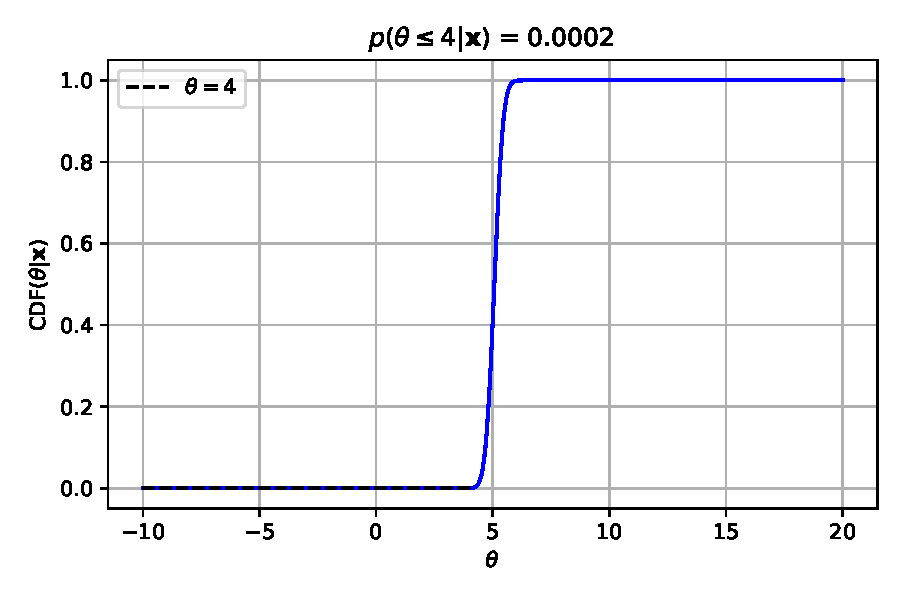
\includegraphics[width=\textwidth]{Q1a_7a.pdf}
         \caption{$F_{\theta \vert \mathbf{x}}(\theta)$.}
     \end{subfigure}
     ~
     \begin{subfigure}[b]{0.45\textwidth}
         \centering
         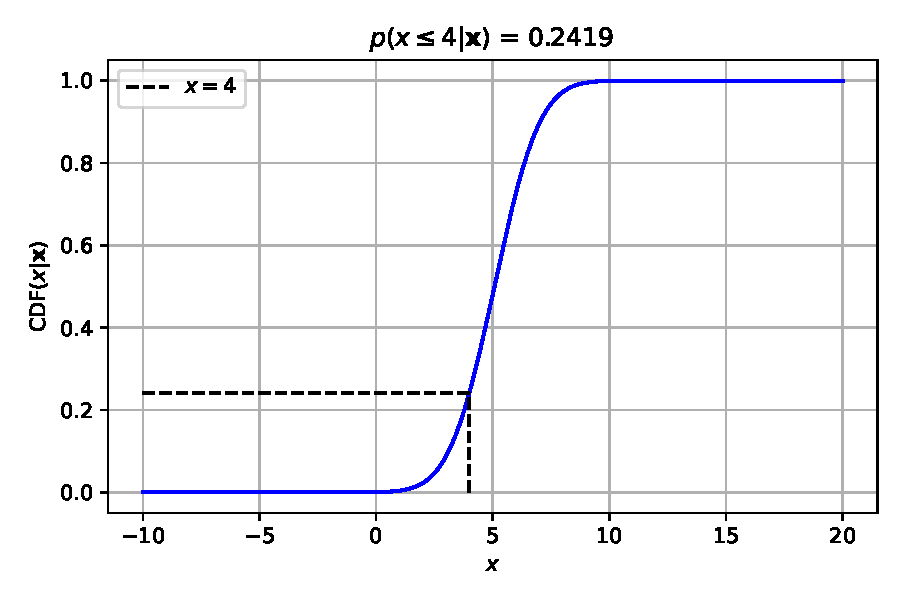
\includegraphics[width=\textwidth]{Q1a_7b.pdf}
         \caption{$F_{x \vert \mathbf{x}}(x)$.}
     \end{subfigure}
     
     \caption{The CDFs used to determine the probabilities $p(\theta \leq 4 \vert \mathbf{x})$ and $p(x \leq 4 \vert \mathbf{x})$ over the domain $\theta \in [-10, 20]$. In a) the CDF of the posterior distribution $p(\theta \vert \mathbf{x})$ is shown, while in b) the CDF of the posterior predictive distribution $p(x \vert \mathbf{x})$ is shown.}
     \label{fig:Q1a_CDFs}
\end{figure}

\subsubsection{Prior hyper-parameters}
At this point in the assignment we have assumed that the prior parameters are fixed in nature. However, there are no set values that are always given to these parameters. As such, all of the distributions of interest in Bayesian inference are conditioned on these parameters. Changing the mean of the prior distribution may be a biased procedure as we are effectively biasing the model towards a certain direction. While this is not always a bad decision, we can also control the impact of the prior in the Bayesian inference process using the prior variance. The prior is parametrised as 
\begin{equation}
p(\theta; \alpha) = L(\theta \vert 0, \alpha)
\end{equation}
where $\alpha$ is a hyper-parameter. The prior hyper-parameter is noticeably influential in posterior distribution
\begin{equation}
p(\theta \vert \mathbf{x}, \alpha) = \frac{p(\mathbf{x}\vert \theta)p(\theta \vert \alpha)}{p(\mathbf{x} \vert \alpha)},
\end{equation}
and the model evidence
\begin{equation}
\begin{aligned}[b]
p(\mathbf{x}) &= \int_\theta p(\mathbf{x}, \theta) d\theta \\
&= \int_\theta p(\mathbf{x} \vert \theta) p(\theta \vert \alpha) d\theta.
\end{aligned}
\end{equation}
As such, a range of $\alpha$ values were considered and the effects on the posterior distribution, the MAP estimate and the model evidence were inspected. In Figure \ref{fig:Q1a_alpha_variation} the results of varying $\alpha$ is shown. It is clear from Figure \ref{fig:Q1a_alpha_variation}b) that by increasing the variance we approach a region where the MAP estimate steadies out. Furthermore, as seen in Figure \ref{fig:Q1a_alpha_variation}d) a larger variance produces a posterior distribution with smaller variation. It is clear that small model variances strongly affect the Bayesian inference process. This implies that having a `tight' prior increases its influence in the results, whereas a prior with a larger variance decreases its influence.
\begin{figure}[htb!]
     \centering
     \begin{subfigure}[b]{0.45\textwidth}
         \centering
         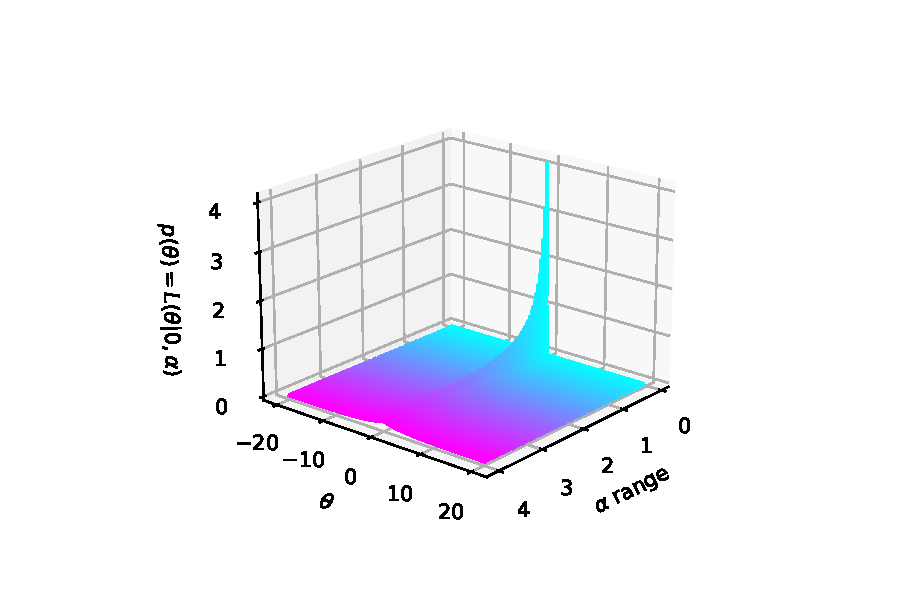
\includegraphics[width=\textwidth]{Q1a_8.pdf}
         \caption{$p(\theta \vert \alpha)$.}
     \end{subfigure}
     ~
     \begin{subfigure}[b]{0.45\textwidth}
         \centering
         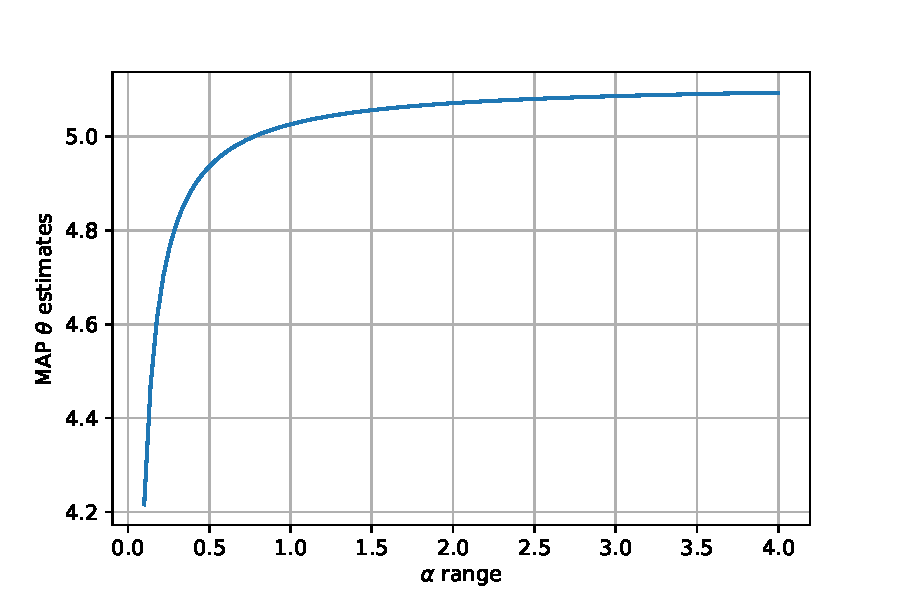
\includegraphics[width=\textwidth]{Q1a_9.pdf}
         \caption{MAP $\theta$ variation.}
     \end{subfigure}
     
     \begin{subfigure}[b]{0.45\textwidth}
         \centering
         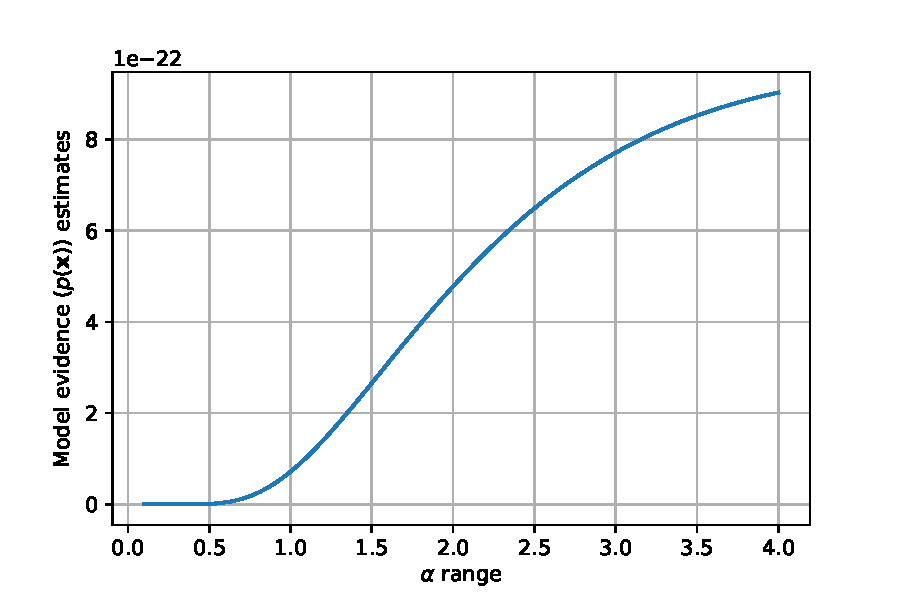
\includegraphics[width=\textwidth]{Q1a_10.pdf}
         \caption{Evidence $p(\mathbf{x})$ variation.}
     \end{subfigure}
     ~
     \begin{subfigure}[b]{0.45\textwidth}
         \centering
         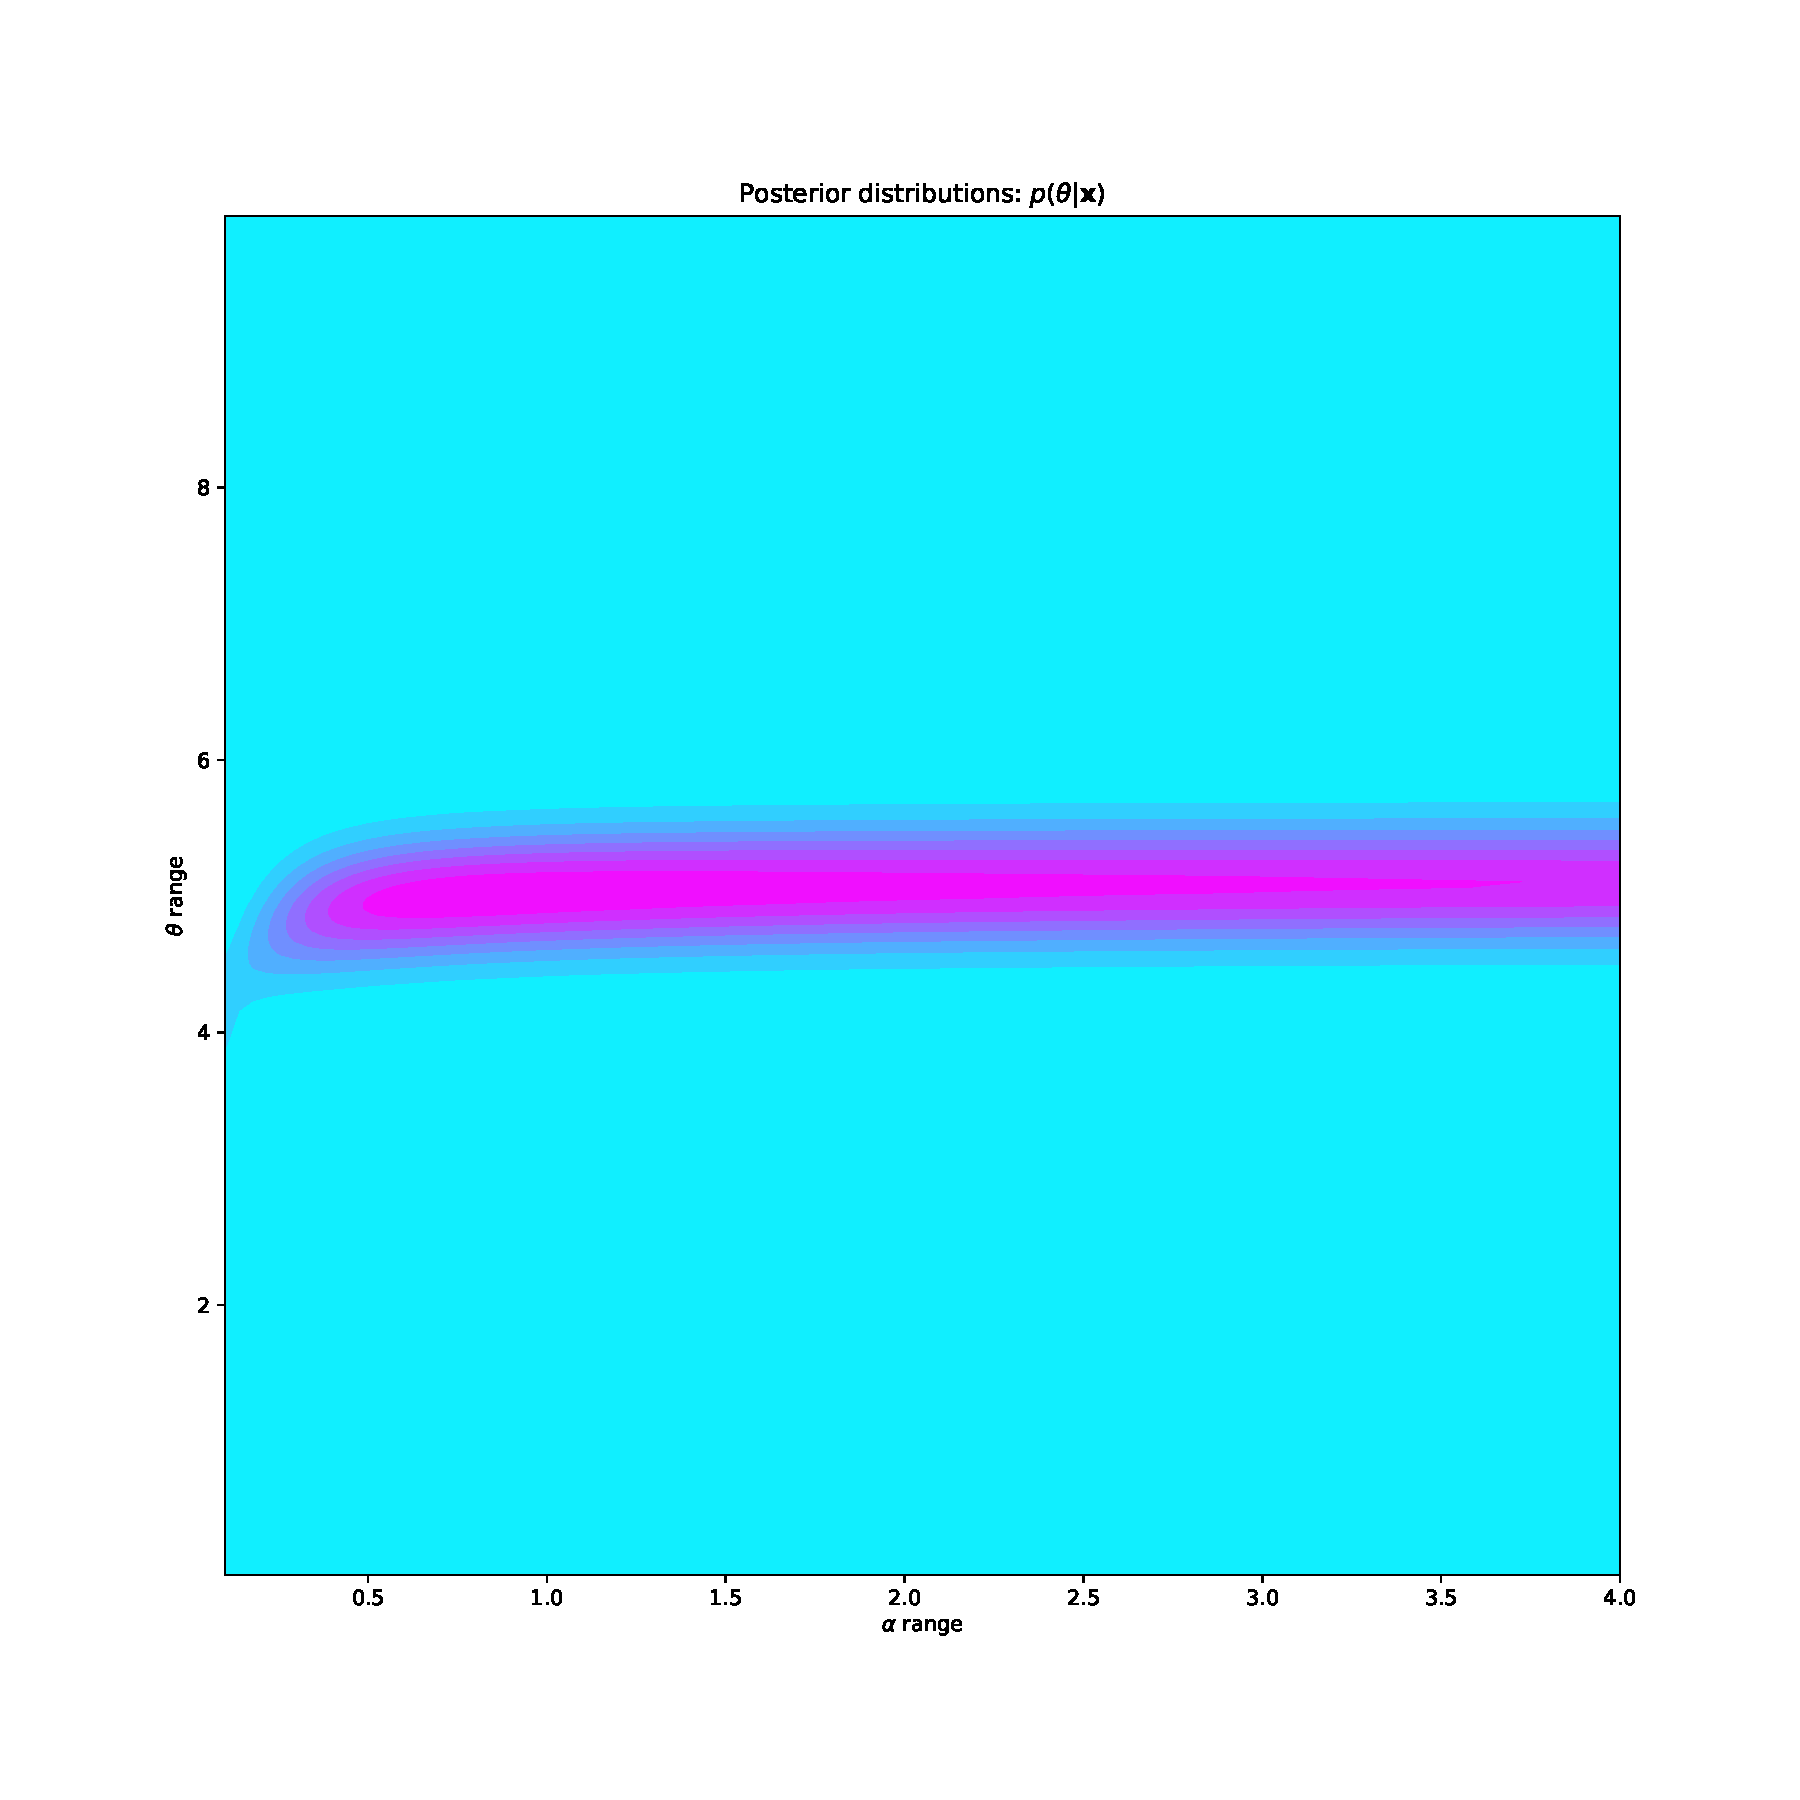
\includegraphics[width=\textwidth]{Q1a_12.pdf}
         \caption{Posterior $p(\theta \vert \mathbf{x})$ variation.}
     \end{subfigure}
     
     \caption{The influence of the prior variance $p(\theta \vert \alpha) = L(\theta \vert 0, \alpha)$ on the Bayesian inference process. In a) the prior is visualised over $\alpha$, in b) the variation of the MAP estimate for $\theta$ is shown, in c) the model evidence variation in shown, and in d) the variation of the posterior $p(\theta \vert \mathbf{x})$ is shown.}
     \label{fig:Q1a_alpha_variation}
\end{figure}


\subsection{Part B: Conjugate Bayesian inference}
Assume that both the parameter $\theta$ and the noise variance $\sigma^2$ are unknowns in the following model
\begin{equation}\label{eq:Q1b_model}
x_n = \theta  + \epsilon_n,
\end{equation}
where $\epsilon_n \sim \mathcal{N}(0, \sigma^2)$. The objective here is to perform Bayesian inference on the unknown model parameters. To assist this process, conjugate priors will be used to improve the posterior condition inference process. We could use specific priors (informative or uninformative priors), or we could use conjugate priors that are specifically designed for the assumed generative model. For this assignment, the form of the generative model is assumed, and a conjugate prior for the unknown model parameters will be used. The generative model is a Gaussian model with unknown mean $\theta$ and precision $\lambda = \sigma^{-2}$. This is given as 
\begin{equation}
p(x \vert \theta, \lambda) = \mathcal{N}(x \vert \theta, \lambda^{-1}) = \left( \frac{\lambda}{2 \cdot \pi} \right)^{\frac{1}{2}} \cdot \exp\left( -\frac{\lambda}{2} \cdot \left( x - \theta \right)^2 \right).
\end{equation}

The assumed generative model, in the presence of some observed data $\mathbf{x} = \left[x_1, \cdots, x_N \right]^T$ comprising of $N$ samples, which gives rise the the likelihood function
\begin{equation}
\begin{aligned}[b]
p(\mathbf{x} \vert \theta, \lambda) &= \prod_{n=1}^{N} p(x_n \vert \theta, \lambda^{-1}) \\
&= \left(\frac{\lambda}{2 \cdot \pi}\right)^{\frac{N}{2}} \cdot \exp \left( -\frac{\lambda}{2} \sum_{n=1}^{N} \cdot \left( x_n - \theta \right)^2 \right).
\end{aligned}
\end{equation}
The likelihood function is proportional to
\begin{equation}\label{eq:Q1b_proportion}
p(\mathbf{x} \vert \theta, \lambda) \propto \left[ \lambda^{\frac{1}{2}} \cdot \exp \left( -\frac{\lambda \cdot \theta^2}{2} \right)\right]^{N} \cdot \left[ \exp \left( - \frac{\lambda}{2} \cdot \sum_{n=1}^{N} x_n^2 + \lambda \cdot \theta \cdot \sum_{n=1}^{N}x_n \right) \right],
\end{equation}
where the normalisation constant $\left(\frac{1}{2 \cdot \pi}\right)^{\frac{N}{2}}$ has been removed. To design a conjugate prior to the assumed likelihood function, we need to construct a prior $p(\theta, \lambda)$ that creates a functionally similar posterior distribution. Before the proceed, we need to think about the domains of $\theta$ and $\sigma^2$. $\theta$ can be any value on the real domain $\mathbb{R}$, while the domain of $\sigma$ (and equivalently, $\lambda$) is bounded to $[0, \infty]$. Thus, the prior distribution should reflect this domain variation. Furthermore, based on the inspection of Equation \eqref{eq:Q1b_proportion}, the prior distribution can be expressed as $p(\theta \vert \lambda)p(\lambda)$. In \citeauthor*{bishop2006} \cite{bishop2006}, the prior of interest given as is the normal-Gamma distribution
\begin{equation}
p(\theta , \lambda) = \mathcal{N}\left( \theta \vert \theta_0, (\beta_0 \cdot \lambda)^{-1} \right)\text{Gam}\left( \lambda \vert a_0, b_0 \right),
\end{equation}
where the Gamma distribution $\text{Gam}\left( \lambda \vert a_0, b_0 \right)$ is given as
\begin{equation}
\text{Gam}\left( \lambda \vert a_0, b_0 \right) = \frac{1}{\Gamma(a_0)} \cdot b_{0}^{a_0} \cdot \lambda^{a_0 - 1} \cdot \exp \left( - b_0 \cdot \lambda \right),
\end{equation}
where the Gamma function $\Gamma(x)$ is given as
\begin{equation}
\Gamma(x) = \int_{0}^{\infty} u^{x - 1} \cdot e^{-u} du.
\end{equation}
Furthermore, the normal distribution $\mathcal{N}\left( \theta \vert \theta_0, (\beta_0 \lambda)^{-1} \right)$ is given as
\begin{equation}
\mathcal{N}\left( \theta \vert \theta_0, (\beta_0 \cdot \lambda)^{-1} \right) = \left(\frac{\beta_0 \cdot \lambda}{2\cdot \pi}\right)^{\frac{1}{2}} \cdot \exp \left(  -\frac{\beta_0 \lambda}{2} \cdot \{ \theta - \theta_0 \}^2\right)
\end{equation}
Thus expanded normal-Gamma distribution is given as
\begin{equation}
p(\theta, \lambda \vert a_0, b_0, \theta_0, \beta_0) = \frac{b_0^{a_0} \cdot \lambda^{\left(a_0 - \frac{1}{2} \right)} \cdot \beta_0^{\frac{1}{2}} }{\Gamma(a_0) \sqrt{2 \cdot \pi}} \exp \left( -\frac{\beta_0 \lambda}{2} \cdot \{ \theta - \theta_0 \}^2 - b_0 \cdot \lambda \right).
\end{equation}
To produce the posterior distribution and posterior-predictive distribution, the emperical mean $\hat{x}$ is
\begin{equation}
\hat{x} = \frac{1}{N} \sum_{n=1}^{N} x_n,
\end{equation}
where this mean is used to condense some of the results that follow. The posterior distribution $p(\theta, \lambda \vert \mathbf{x})$ is given as
\begin{equation}
p(\theta, \lambda \vert \mathbf{x}) = NG(\theta, \lambda \vert a_n, b_n, \theta_n, \beta_n) = N(\theta \vert \theta_n, \left( \beta_n \cdot \lambda \right)^{-1}) \text{Gam}\left( \lambda \vert a_n, b_n \right),
\end{equation}
where
\begin{equation}\label{eq:theta_update}
\theta_n = \frac{\beta_0 \theta_0 + N \cdot \hat{x}}{\beta_0 + N},
\end{equation}
\begin{equation}\label{eq:beta_update}
\beta_n = \beta_0 + N,
\end{equation}
\begin{equation}\label{eq:a_update}
a_n = a_0 + \frac{N}{2},
\end{equation}
\begin{equation}\label{eq:b_update}
b_n = b_0 + \frac{1}{2}\sum_{n=1}^{N}(x_i - \hat{x})^2 + \frac{\beta_0 \cdot N \cdot (\hat{x} - \theta_0)^2}{2 \cdot (\beta_0 + N)}.
\end{equation}


Additionally, the posterior marginal distributions are given as
\begin{equation}\label{eq:Q1b_marginal_theta}
p(\theta \vert \mathbf{x}) = T_{2 \cdot a_n} \left( \theta \vert \theta_n, \frac{b_n}{a_n \cdot \beta_n} \right),
\end{equation}
\begin{equation}\label{eq:Q1b_marginal_lambda}
p(\lambda \vert \mathbf{x}) \text{Gam}(\theta \vert a_n, b_n),
\end{equation}
where $t_\nu(x \vert \mu, \sigma^2)$ is a Student-t distribution
\begin{equation}
t_\nu(x \vert \mu, \sigma^2) = c \left[ 1 + \frac{1}{\nu} \cdot \left(\frac{x - \mu}{\sigma} \right)^2 \right]^{-\left( \frac{\nu + 1}{2} \right)},
\end{equation}
where $\nu$ is the degrees of freedom. The parameter $c$ is given as
\begin{equation}
c = \frac{\Gamma \left(\frac{\nu}{2} + \frac{1}{2}\right)}{\Gamma \left(\frac{\nu}{2}\right)} \cdot \frac{1}{\sqrt{\nu \cdot \pi \cdot \sigma^2}}.
\end{equation}

The posterior predictive distribution is given as
\begin{equation}\label{eq:Q1b_posterior_predict}
p(x \vert \mathbf{x}) = T_{2 \cdot a_n} \left(x \vert \theta_n, \frac{b_n \cdot \left( \beta_n + 1 \right)}{a_n \cdot \beta_n}  \right).
\end{equation}

\subsubsection{Maximum likelihood estimation}
Given the generative model in Equation \eqref{eq:Q1b_model} and the observed data shown in Figure \ref{fig:Q1_data}, we can obtain maximum likelihood estimates for the unknown model parameters $\theta$ and $\sigma$. 
These are given through
\begin{equation}
\begin{aligned}[b]
\hat{\theta} &= \frac{1}{N} \sum_{n=1}^{N} x_n \\
&= 5.1161,
\end{aligned}
\end{equation}
\begin{equation}
\begin{aligned}[b]
\hat{\sigma} &= \frac{1}{N} \sum_{n=1}^{N} (x_n - \overline{\theta})^2 \\
&= 1.3905 \\
\lambda &= \frac{1}{\hat{\sigma}^2} = 0.5172.
\end{aligned}
\end{equation}

\subsubsection{Bayesian inference}
In this problem, we will use the Normal-Gamma conjugate prior to perform Bayesian inference for the generative model parameters $\theta$ and $\lambda$. In this investigation, the prior will be explored, and from this an investigation will be performed into how the prior hyper-parameters affect the MAP estimates will be conducted. This is to ensure that reasonable parameter ranges are selected and to determine the sensitivity of the Bayesian inference process to the prior.

\subsubsection*{The prior distribution}
To gain some intuition into how the prior parameters affect the Normal-Gamma prior, different initialisations of the prior is needed. In Figure \ref{fig:Q1b_prior} different initialisations of the prior are shown. It is clear that $a$ and $b$ affect the distribution in the $\lambda$ direction, while $\theta_0$ and $\beta_0$ affect the mean and spread along the $\theta$ dimension.
\begin{figure}[htb!]
     \centering
     \begin{subfigure}[b]{0.7\textwidth}
         \centering
         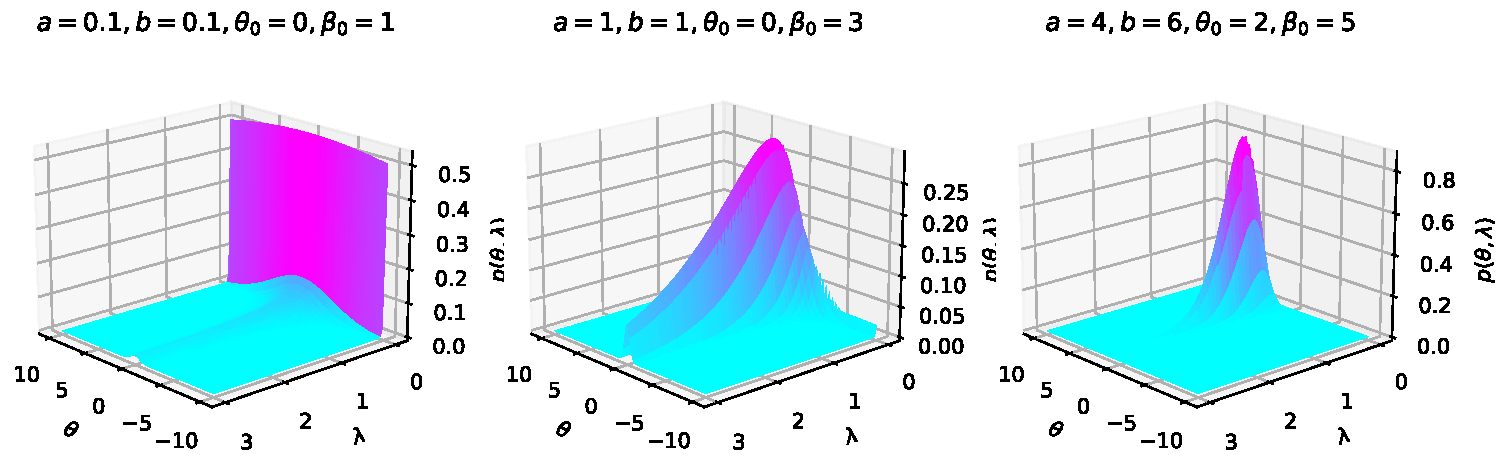
\includegraphics[width=\textwidth]{Q1b_1.pdf}
         \caption{Three-dimensional visualisation.}
     \end{subfigure}
     
     \begin{subfigure}[b]{0.7\textwidth}
         \centering
         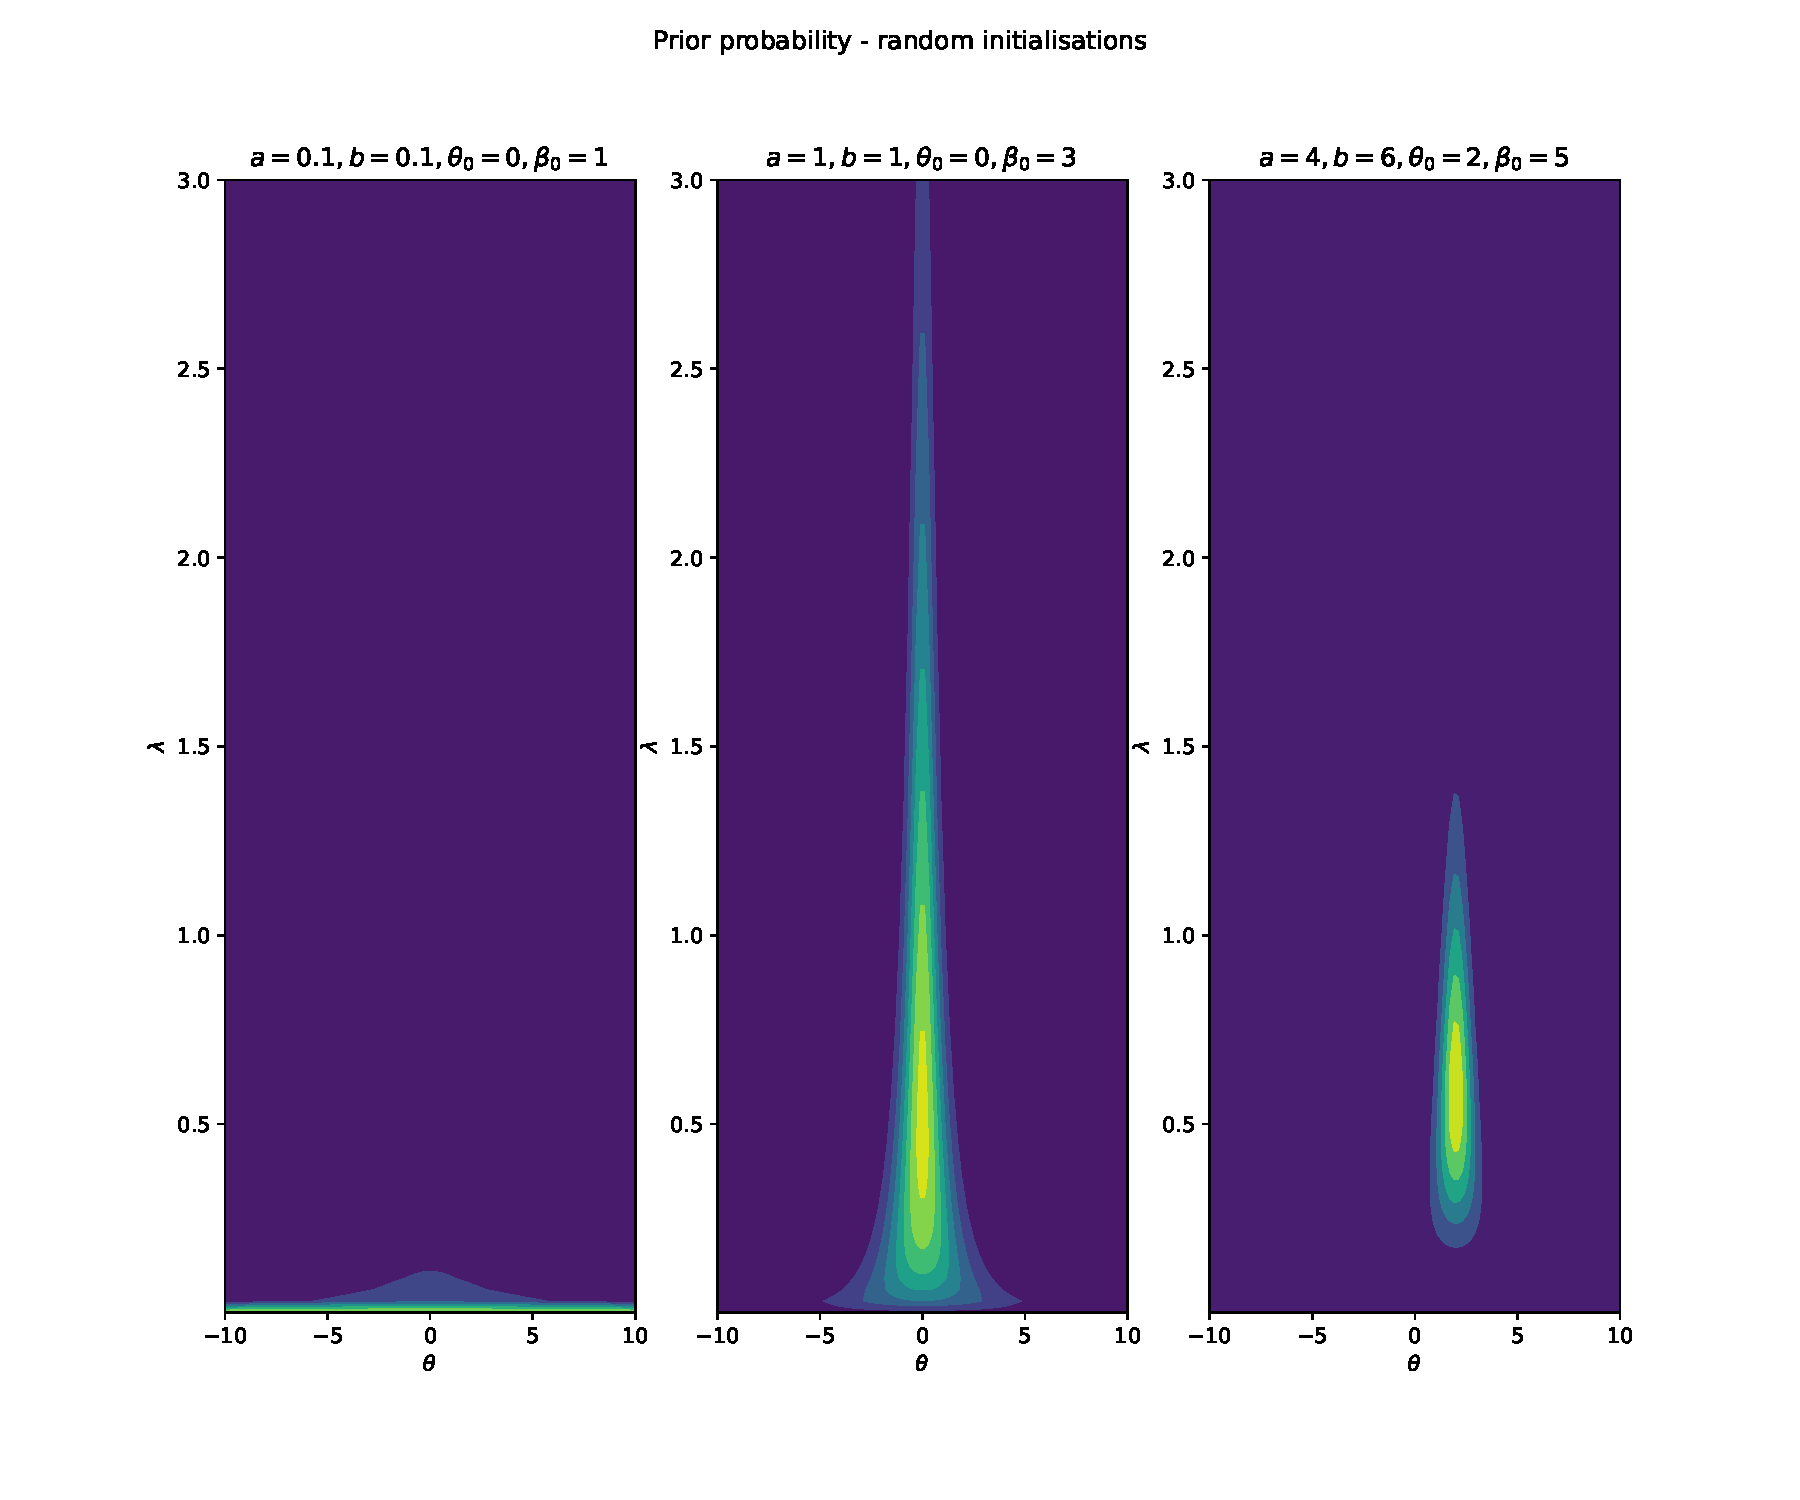
\includegraphics[width=\textwidth]{Q1b_2.pdf}
         \caption{Two-dimensional visualisation.}
     \end{subfigure}
     
     \caption{The Normal-Gamma prior under different hyper-parameter initialisations.}
     \label{fig:Q1b_prior}
\end{figure}

\subsubsection*{Prior hyper-parameter investigation}
To conduct than investigation into the prior hyper-parameters, a reference prior state was used and each parameter was perturbed individually. The initial parameter state was set to $a_0 = 1, b_0 = 1, \theta_0 = 0, \lambda_0 = 3$. This was chosen at it gives a subjectively reasonable spread in each hyper-parameter dimension. This prior is visualised in Figure \ref{fig:Q1b_initial_prior}.
\begin{figure}[htb!]
     \centering
     \begin{subfigure}[b]{0.45\textwidth}
         \centering
         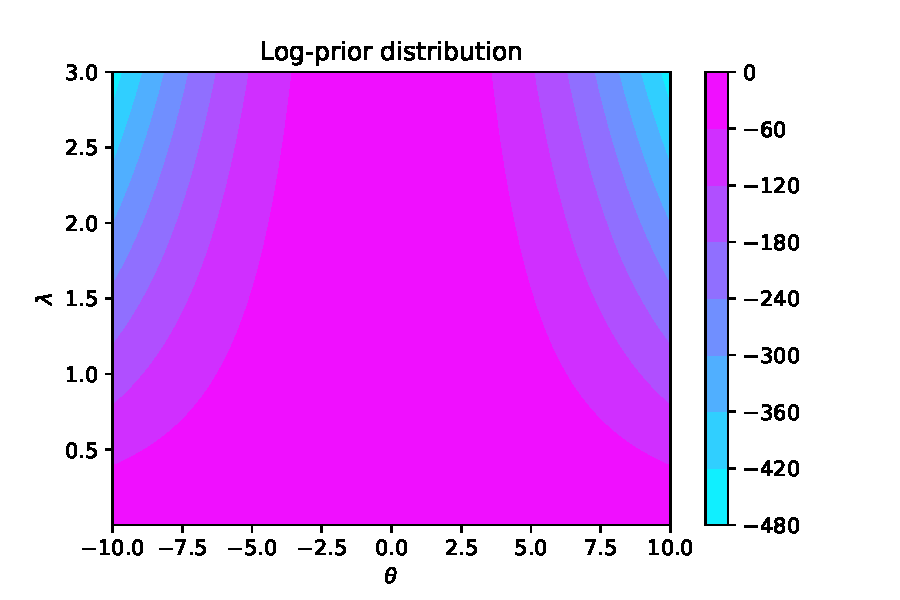
\includegraphics[width=\textwidth]{Q1b_3.pdf}
         \caption{log-prior.}
     \end{subfigure}
     ~
     \begin{subfigure}[b]{0.45\textwidth}
         \centering
         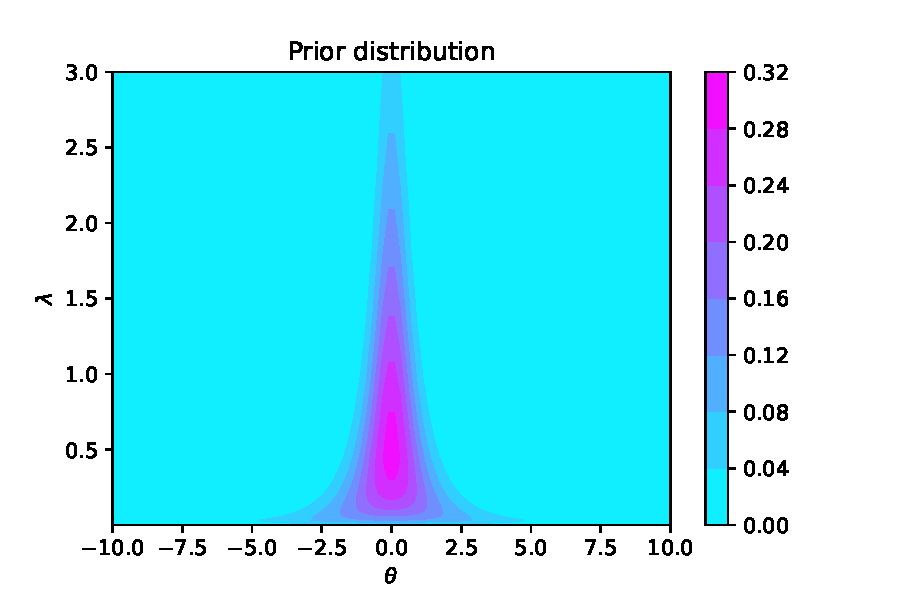
\includegraphics[width=\textwidth]{Q1b_4.pdf}
         \caption{prior.}
     \end{subfigure}
     
     \caption{The log Normal-Gamma prior and the Normal-Gamma prior in its initial state. The initial parameters are: $a_0 = 1, b_0 = 1, \theta_0 = 0, \lambda_0 = 3$.}
     \label{fig:Q1b_initial_prior}
\end{figure}

In Figure \ref{fig:Q1b_param_invest} the results from the prior hyper-parameter investigation is shown. It is clear from Figure \ref{fig:Q1b_param_invest} that the MAP estimates, and thus the posterior distribution, exhibits a large sensitivity to $\theta_0$ and $\beta_0$. While the MAP estimates under a perturbation of $a_0$ and $b_0$ result in some changes, but to a lesser extent. In the perturbation of $\theta_0$, it is interesting to note that as the $\theta$ hyper-parameter is perturbed to approach the ML estimate, the $\lambda$ MAP estimate also approaches the ML $\lambda$ estimate. Furthermore, as seen in Figure \ref{fig:Q1b_param_invest}, perturbations of $\beta_0$ result in significant MAP parameter estimate variation.
\begin{figure}[htb!]
\centering
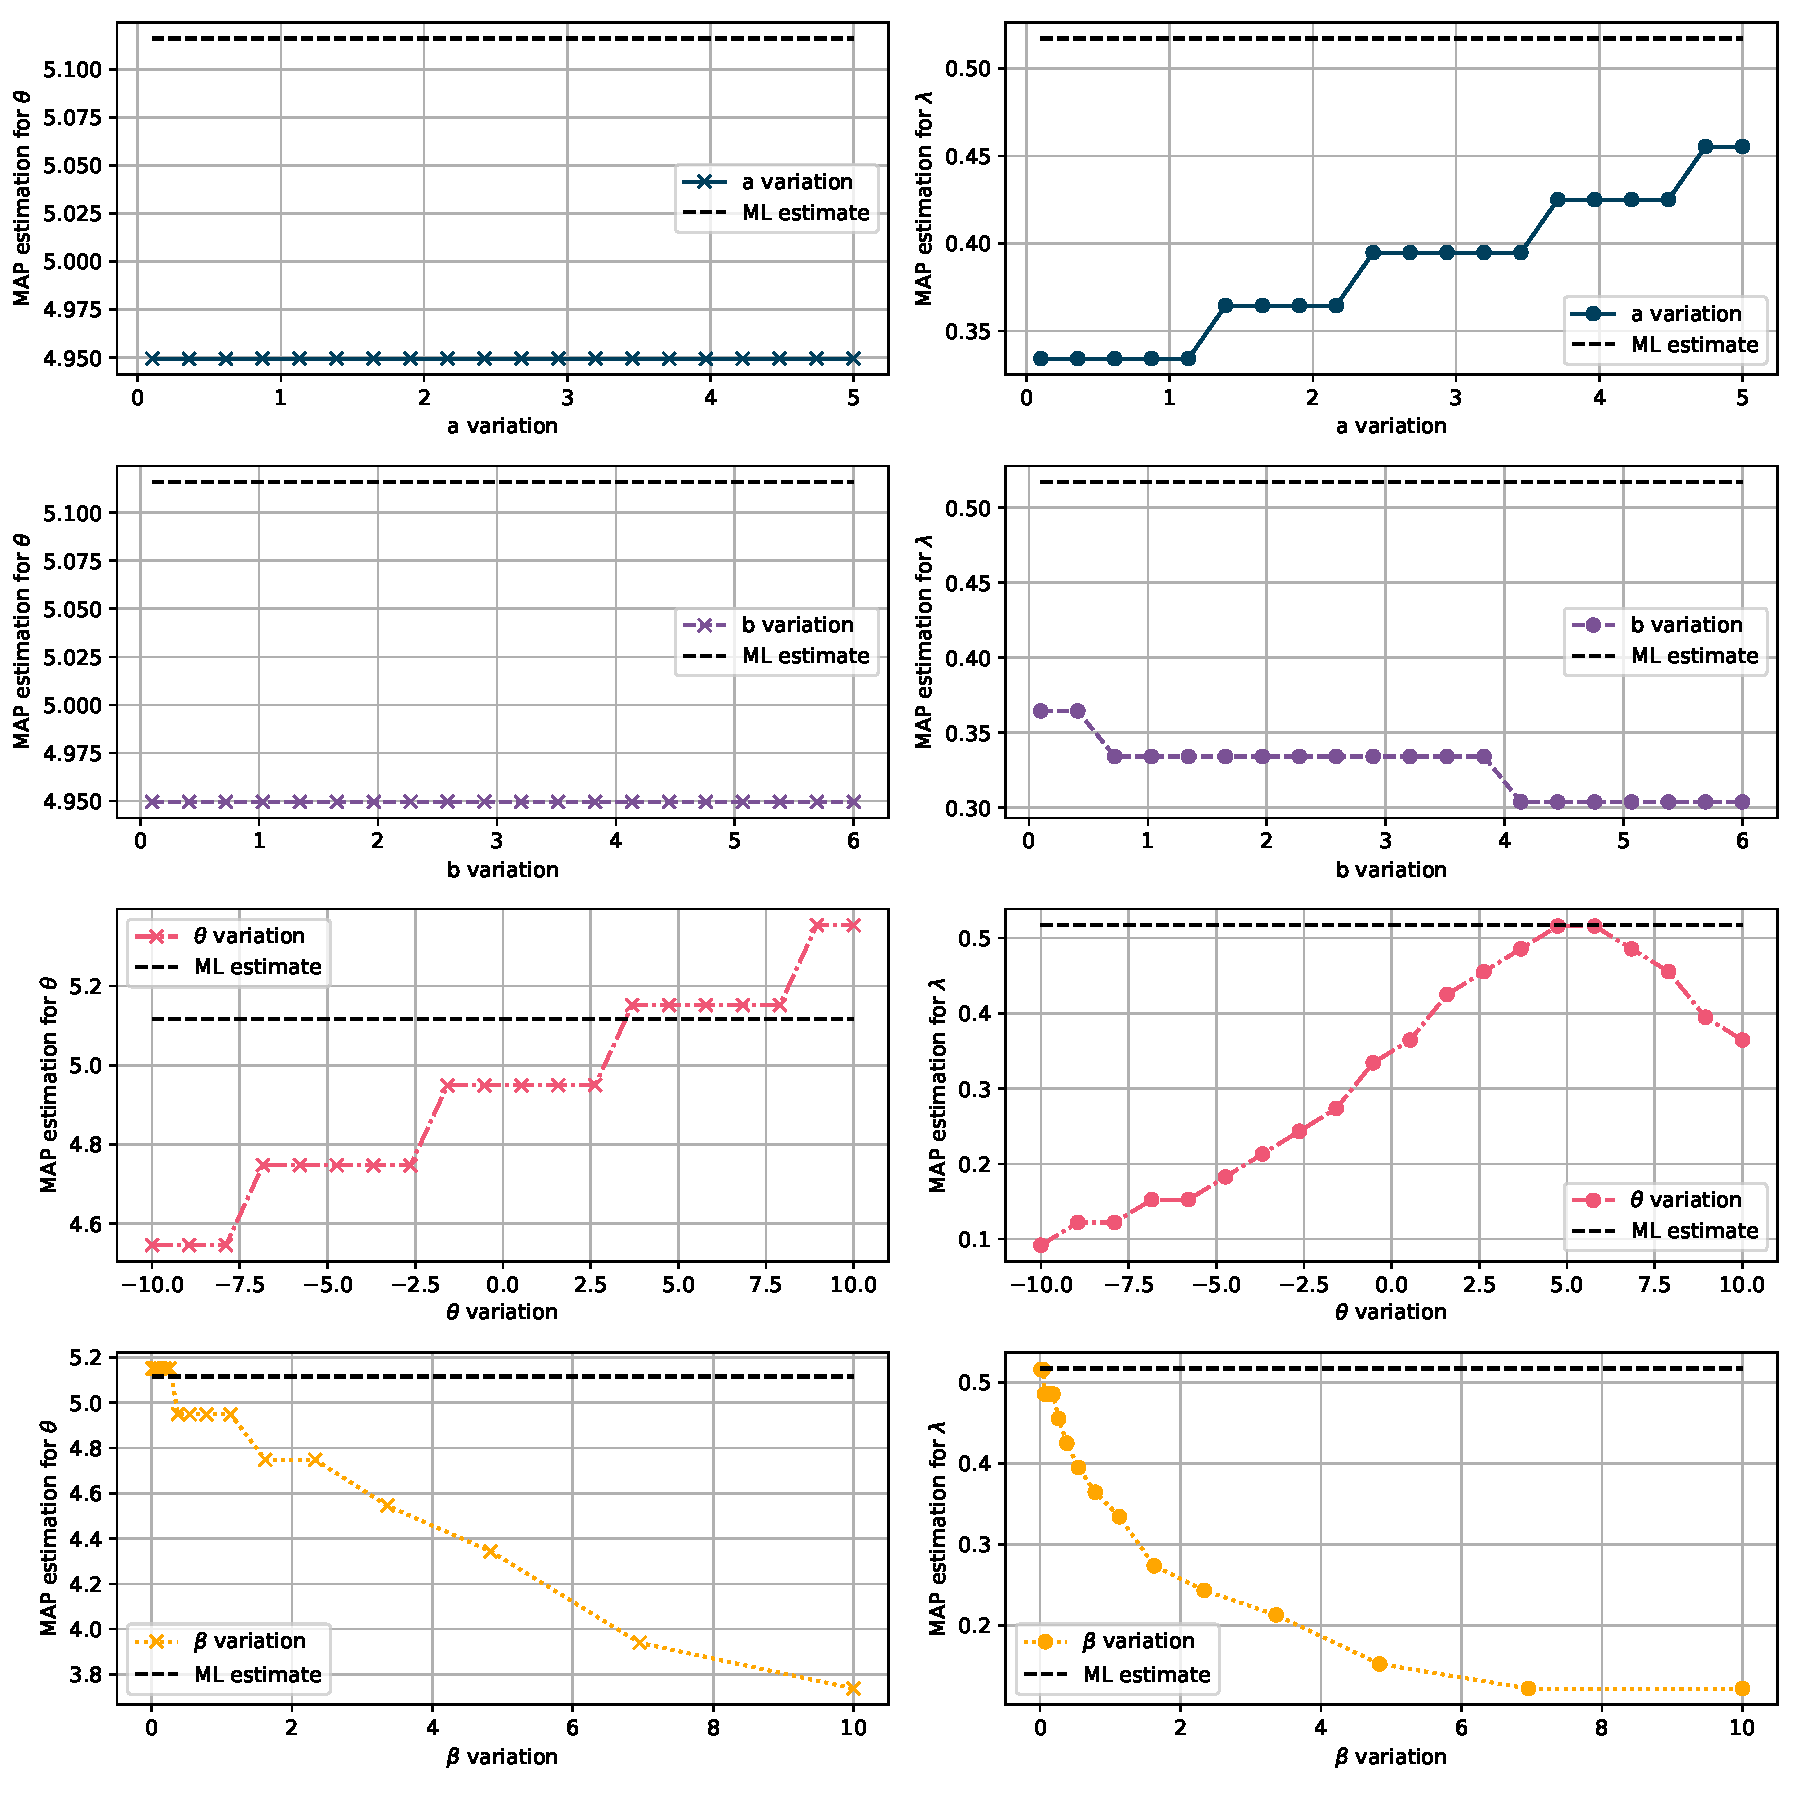
\includegraphics[scale=0.5]{Q1b_5.pdf}
\caption{The resulting MAP estimates for $\theta$ and $\lambda$ for each of the prior hyper-parameters.}
\label{fig:Q1b_param_invest}
\end{figure}

\subsubsection*{Inference results}
Equations \eqref{eq:theta_update}, \eqref{eq:beta_update}, \eqref{eq:a_update}, and \eqref{eq:b_update} were used to obtain the hyper-parameters of the posterior Normal-Gamma distribution. In Table \ref{tab:Q1_b} the prior and updated hyper-parameters are shown. Note that the $\lambda_0$ parameter was reduced so that its effect was less pronounced. Naturally, decreasing $\lambda_0$ is akin to raising the variance of a Gaussian distribution. This was done to reduce to dominance of the prior in the resulting posterior distribution. 
In Table \ref{tab:Q1_c} the MAP estimates for the unknown parameters are shown. It is clear that there are significant changes in the posterior distribution parameters. In Figure \ref{fig:Q1b_prior_posterior} the prior and posterior distributions with parameters given in Table \ref{tab:Q1_c} are given. It is clear from Figure \ref{fig:Q1b_prior_posterior} that the posterior distribution is highly localised around the MAP parameters. 
\begin{table}[htb!]
\centering
\caption{The estimates for the hyper-parameters of the prior and posterior Normal-Gamma distributions}
\label{tab:Q1_b}
\begin{tabular}{@{}ccccc@{}}
\toprule
 & $a$ & $b$ & $\theta$ & $\lambda$ \\ \midrule
Prior parameters & 2 & 3 & 0 & 0.1 \\
Posterior parameters & 14.5 & 28.473 & 5.096 & 25.1 \\ \bottomrule
\end{tabular}
\end{table}

\begin{table}[]
\centering
\caption{The estimates for the model parameters $\theta$ and $\lambda$ using maximum likelihood and maximum a posteriori estimation. The MAP estimates were found through numerical optimisation.}
\label{tab:Q1_c}
\begin{tabular}{@{}ccc@{}}
\toprule
Parameter & Maximum likelihood & MAP \\ \midrule
$\theta$ & 5.116 & 5.0957 \\
$\lambda$ & 0.5172 & 0.4917 \\
$\sigma$ & 1.3905 & 1.4261 \\ \bottomrule
\end{tabular}
\end{table}

\begin{figure}[htb!]
     \centering
     \begin{subfigure}[b]{0.45\textwidth}
         \centering
         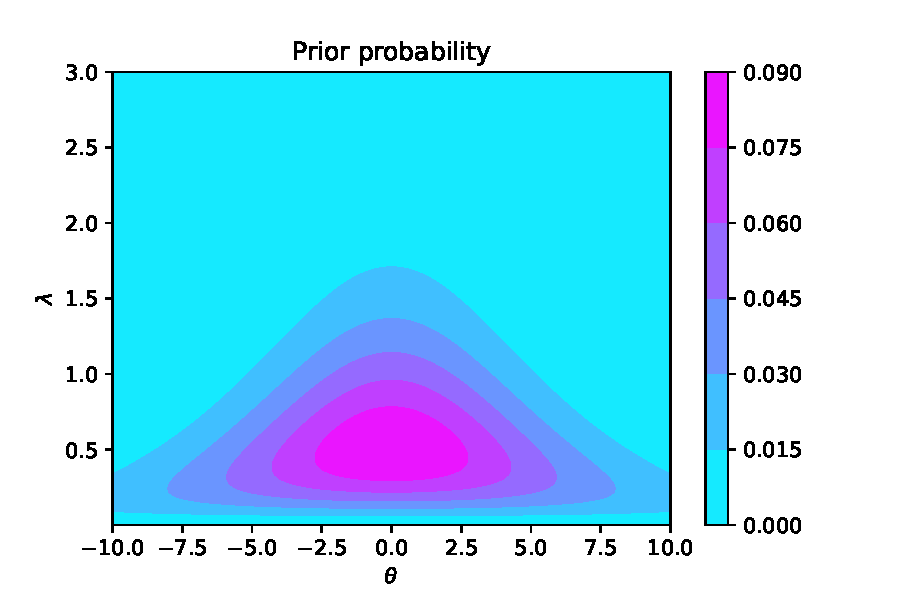
\includegraphics[width=\textwidth]{Q1b_9.pdf}
         \caption{Prior distribution $p(\theta, \lambda)$.}
     \end{subfigure}
     ~
     \begin{subfigure}[b]{0.45\textwidth}
         \centering
         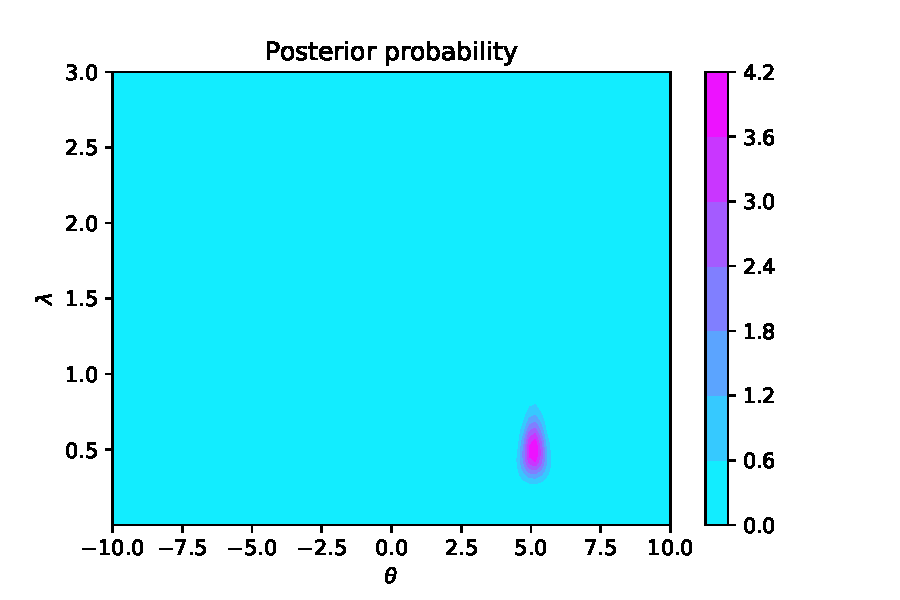
\includegraphics[width=\textwidth]{Q1b_11.pdf}
         \caption{Posterior distribution $p(\theta, \lambda \vert \mathbf{x})$.}
     \end{subfigure}
     
     \caption{The prior and posterior Normal-Gamma distributions. The parameters for these distributions are given in Table \ref{tab:Q1_b}.}
     \label{fig:Q1b_prior_posterior}
\end{figure}

The Bayesian inference process allows us to inspect the posterior distribution over $\theta$ and $\lambda$, and through marginalisation we can inspect the posterior marginal distribution $p(\theta \vert \mathbf{x})$ and $p(\lambda \vert \mathbf{x})$. In Figure \ref{fig:Q1b_marginals} these distributions are shown. Note that Equations \eqref{eq:Q1b_marginal_theta} and \eqref{eq:Q1b_marginal_lambda} were used to develop Figure \ref{fig:Q1b_marginals}. Using Equation \eqref{eq:Q1b_posterior_predict}, the posterior predictive distribution was determined. In Figure \ref{fig:Q1b_post_predict} the posterior predictive distribution is shown. 
\begin{figure}[htb!]
     \centering
     \begin{subfigure}[b]{0.45\textwidth}
         \centering
         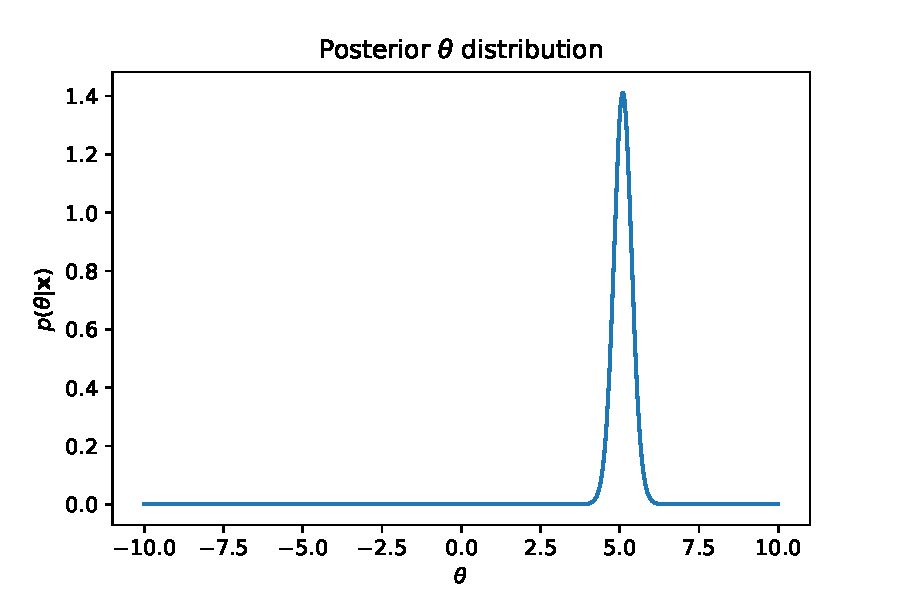
\includegraphics[width=\textwidth]{Q1b_12.pdf}
         \caption{$p(\theta \vert \mathbf{x})$.}
     \end{subfigure}
     ~
     \begin{subfigure}[b]{0.45\textwidth}
         \centering
         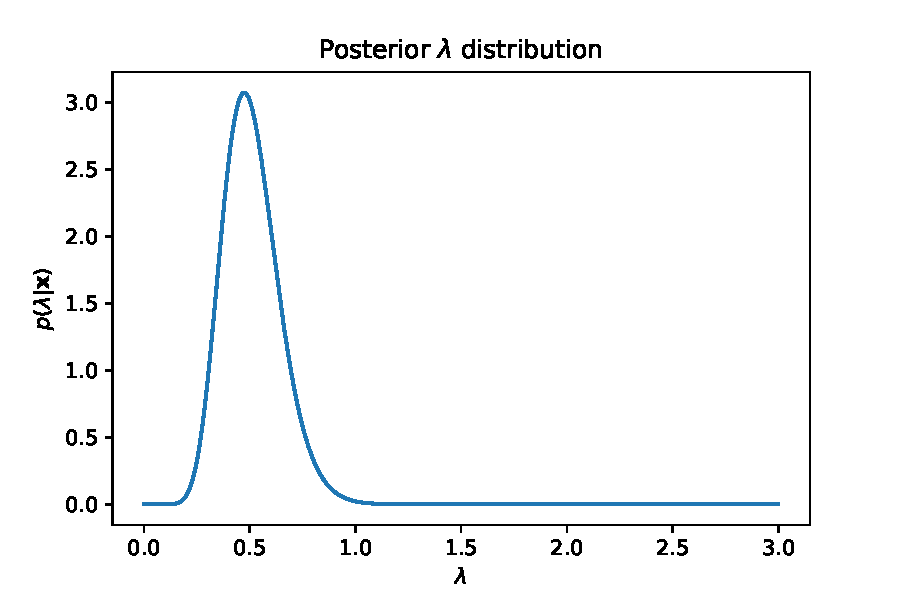
\includegraphics[width=\textwidth]{Q1b_13.pdf}
         \caption{$p(\lambda \vert \mathbf{x})$.}
     \end{subfigure}
     
     \caption{The posterior marginal distributions for $\theta$ and $\lambda$.}
     \label{fig:Q1b_marginals}
\end{figure}

\begin{figure}[htb!]
\centering
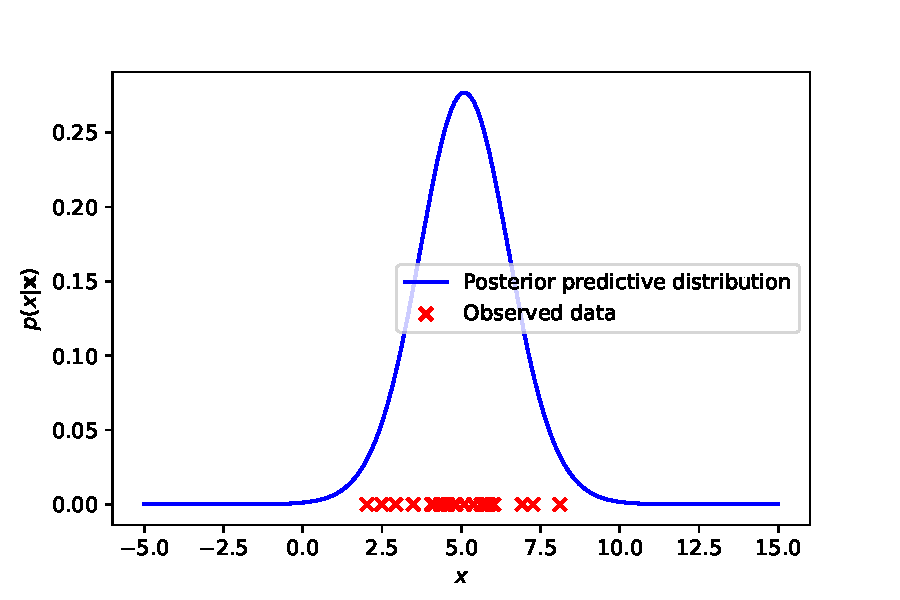
\includegraphics[scale=0.7]{Q1b_14.pdf}
\caption{The posterior predictive distribution $p(x \vert \mathbf{x})$ for the Bayesian conjugate prior inference process.}
\label{fig:Q1b_post_predict}
\end{figure}

\subsubsection*{Using Bayesian inference}
We can use the posterior distribution $p(\theta \vert \mathbf{x})$ and the posterior predictive distribution $p(x \vert \mathbf{x})$ to determine probabilities $p(a \leq X \leq b)$. The first probability of interest is $p(\theta \leq 4 \vert \mathbf{x})$ and the second is $p(x \leq 4 \vert \mathbf{x})$. It was found that $p(\theta \leq 4 \vert \mathbf{x}) = 0.0003$ and $p(x \leq 4 \vert \mathbf{x}) = 0.2247$. In Figure \ref{fig:Q1b_CDFs} the CDFs of interest and the resulting probabilities are shown. The posterior probability that $\theta \leq 4$ informs us that it is very unlikely that a model parameter $\theta$ in this range is responsible for generating the observed data. The posterior predictive probability that $x \leq 4$ is noticeably larger, and this indicates that it is far more probable that newly observed $x$ samples may be drawn in the $x$ domain $x \in [-\infty, 4]$. 
\begin{figure}
     \centering
     \begin{subfigure}[b]{0.45\textwidth}
         \centering
         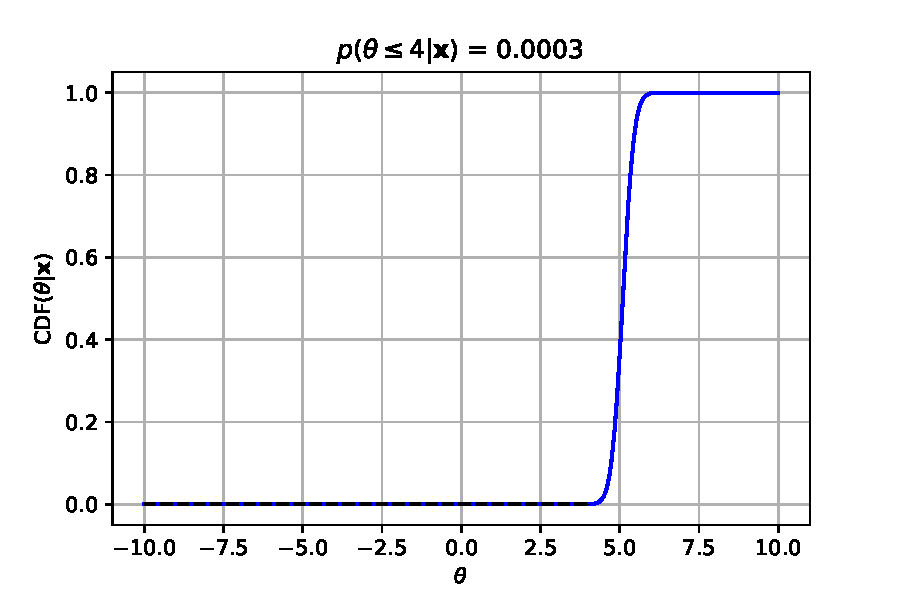
\includegraphics[width=\textwidth]{Q1b_15.pdf}
         \caption{$F_{\theta \vert \mathbf{x}}(\theta)$.}
     \end{subfigure}
     ~
     \begin{subfigure}[b]{0.45\textwidth}
         \centering
         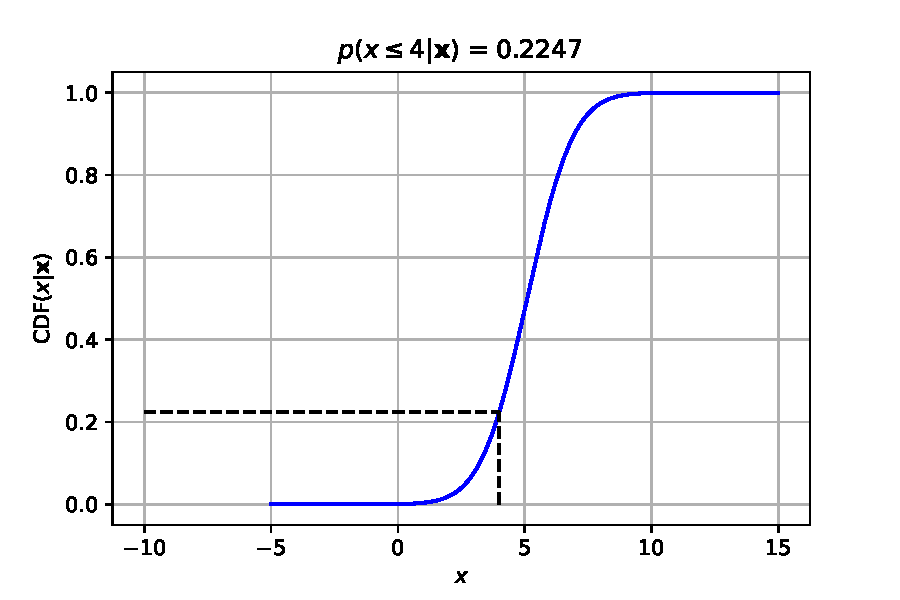
\includegraphics[width=\textwidth]{Q1b_16.pdf}
         \caption{$F_{x \vert \mathbf{x}}(x)$.}
     \end{subfigure}
     
     \caption{The CDFs used to determine the probabilities $p(\theta \leq 4 \vert \mathbf{x})$ and $p(x \leq 4 \vert \mathbf{x})$. In a) the CDF of the posterior distribution $p(\theta \vert \mathbf{x})$ is shown, while in b) the CDF of the posterior predictive distribution $p(x \vert \mathbf{x})$ is shown.}
     \label{fig:Q1b_CDFs}
\end{figure}

\clearpage

\section{Question 2}
Consider the regression model
\begin{equation}
\begin{aligned}[b]
y_n &= f(x_n) + \epsilon_n \\
&= \omega_0 + \omega_1 \cdot x_n + \omega_2 \cdot x_n^2 + \cdots +  + \omega_K \cdot x_n^{K} + \epsilon_n \\
&= \boldsymbol\omega^T \boldsymbol\phi(x_n) + \epsilon_n,
\end{aligned}
\end{equation}
where $y_n$ denotes the regression model response, $x_n$ is the independent regression variable, $\boldsymbol\omega$ is the regression parameter vector, $\boldsymbol\phi(\cdot)$ is a basis column vector and $\epsilon_n$ is the sample noise
\begin{equation}
\epsilon_n \sim \mathcal{N}(0, \sigma^2),
\end{equation}
with $\sigma = 0.5$. As the noise is an additive Gaussian distribution, the generative model is
\begin{equation}
p(y\vert x, \boldsymbol\omega, \sigma^2) = \mathcal{N}(y \vert f(x), \sigma^2).
\end{equation}

In this problem, the goal is to perform Bayesian inference. The conjugate prior for this process is given by
\begin{equation}
p(\boldsymbol\omega) = \mathcal{N}(\boldsymbol\omega \vert \mathbf{0}, \frac{1}{\alpha} \mathbf{I}),
\end{equation}
where $\alpha$ is the prior precision. The observed regression data $\mathbf{y} = [y_1, y_2, \cdots, y_N]^T$ and corresponding independent variable $\mathbf{x} = [x_1, x_2, \cdots, x_N]^T$ is detailed in Figure \ref{fig:Q2_data}.
\begin{figure}[htb!]
\centering
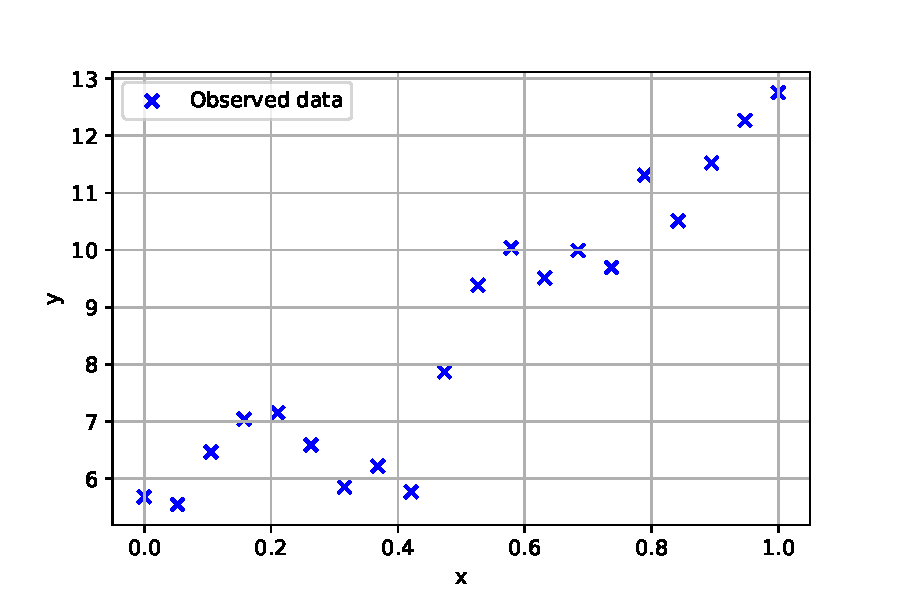
\includegraphics[scale=0.5]{Q2_1.pdf}
\caption{The observed regression data for Question 2.}
\label{fig:Q2_data}
\end{figure}

\subsection{Bayesian inference}

In order to perform Bayesian inference, we assume that the samples in $\mathcal{D}$ satisfy the \emph{i.i.d} assumption. As such, we can calculate the conditional likelihood function $p(\mathbf{y} \vert \mathbf{x})$ as follows
\begin{equation}
p(\mathbf{y} \vert \mathbf{x}, \boldsymbol\omega, \sigma^2) = \prod_{n=1}^{N} p(y_n \vert x_n, \boldsymbol\omega, \sigma^2),
\end{equation}
However, to avoid numerical underflow issues, and to simplify derivative computations, the logarithm of the likelihood function is used, which gives
\begin{equation}
\begin{aligned}[b]
\log p(\mathbf{y} \vert \mathbf{x}, \boldsymbol\omega, \sigma^2) &= \sum_{n=1}^{N} p(y_n \vert x_n) \\
\mathcal{L}(\boldsymbol\omega) &= \sum_{n=1}^{N} \left( -\frac{1}{2}\log \left( 2\pi \right) -\frac{1}{2}\log \left( \sigma^2 \right) - \frac{1}{2\sigma^2} \left[ y_n - f(x_n)\right] ^2 \right), \\
&=  -\frac{N}{2}\log \left( 2\pi \right) -\frac{N}{2}\log \left( \sigma^2 \right) - \frac{1}{2\sigma^2}\sum_{n=1}^{N} \left( \left[ y_n - f(x_n)\right] ^2 \right),
\end{aligned}
\end{equation}

where $\mathcal{L}(\mathbf{w}, \sigma^2)$ is the log-likelihood function that we wish to maximise. To perform maximum likelihood estimation  we would maximise this function, we can use numerous methods (grid search, optimisation), but in this assignment we will make use of the analytical solution to the ML problem. The ML estimate for $\boldsymbol\omega$ is given as
\begin{equation}
\hat{\boldsymbol\omega} = \left( \boldsymbol\Phi^T \boldsymbol\Phi \right)^{-1} \boldsymbol\Phi^T \mathbf{t},
\end{equation}
where 
\begin{equation}
\boldsymbol\Phi = 
\begin{bmatrix}
\phi_1^{(0)} & \phi_1^{(1)} & \cdots & \phi_1^{(K)} \\
\phi_2^{(0)} & \phi_2^{(1)} & \cdots & \phi_2^{(K)} \\
\vdots & \vdots & \ddots & \vdots \\
\phi_N^{(0)} & \phi_N^{(1)} & \cdots & \phi_N^{(K)} \\
\end{bmatrix},
\end{equation}
such that the $n^{th}$ row of $\boldsymbol\Phi$ is equal to $\boldsymbol\phi(x_n)^T$ and $\boldsymbol\Phi \in \mathbb{R}^{N \times K + 1}$. Given the ML estimate for the regression parameters, the sampling distribution of the estimated parameters is given by
\begin{equation}
\hat{\boldsymbol\omega} \sim \mathcal{N}(\boldsymbol\omega_{ML}, \boldsymbol\Sigma_{ML}),
\end{equation}
where the covariance $\boldsymbol\Sigma_{ML}$ is given by
\begin{equation}
\boldsymbol\Sigma_{ML} = \sigma^2 \cdot \left(\boldsymbol\Phi^T \boldsymbol\Phi\right)^{-1}.
\end{equation}
However, in the Bayesian inference setting we are interesting in the posterior distribution $p(\boldsymbol\omega \vert \mathbf{x}, \mathbf{y})$, which is given in \citeauthor*{bishop2006} \cite{bishop2006} as
\begin{equation}
p(\boldsymbol\omega \vert \mathbf{x}, \mathbf{y}) = \mathcal{N}\left(\boldsymbol\omega \vert \boldsymbol\mu_{\boldsymbol\omega}, \boldsymbol\Sigma_{\boldsymbol\omega}  \right),
\end{equation}
where the mean of the multivariate Gaussian posterior distribution is
\begin{equation}
\boldsymbol\mu_{\boldsymbol\omega} = \left( \boldsymbol\Phi^T \boldsymbol\Phi + \frac{\alpha}{\beta}\cdot \mathbf{I}  \right)^{-1} \boldsymbol\Phi^T \mathbf{y},
\end{equation}
and the covariance of the multivariate Gaussian posterior distribution is
\begin{equation}
\boldsymbol\Sigma_{\boldsymbol\omega} = \left( \beta \cdot \boldsymbol\Phi^T \boldsymbol\Phi + \alpha \cdot \mathbf{I}  \right)^{-1}.
\end{equation}
Note that the parameter $\beta$ is the inverse of the generative model variance
\begin{equation}
\beta = \frac{1}{\sigma^2}.
\end{equation}

Furthermore, the posterior predictive distribution is given as
\begin{equation}\label{eq:Q2_post_predict}
p(y \vert x, \mathbf{x}, \mathbf{y}, \alpha, \beta) = \mathcal{N}(y \vert \boldsymbol\mu^{T}_{\boldsymbol\omega} \boldsymbol\phi(x), \sigma_p(x)^2),
\end{equation}
where the posterior predictive variance is given as
\begin{equation}
\sigma_p(x)^2 = \frac{1}{\beta} + \boldsymbol\phi(x)^T \boldsymbol\Sigma_{\boldsymbol\omega}\boldsymbol\phi(x).
\end{equation}

\subsubsection*{The posterior distribution}
The posterior distribution over $\boldsymbol\omega$ is dependent on the polynomial order $K$. For an order of $K = 1$, the posterior mean (which is also the MAP estimate for $\boldsymbol\omega$) is given by
\begin{equation}
\boldsymbol\mu_{\boldsymbol\omega} = 
\begin{bmatrix}
5.6164 & 16.3821 & -119.3896 & 352.7705 & -397.5298 & 154.9652
\end{bmatrix}^T.
\end{equation}
In comparison, the ML estimate for the optimal regression parameters is
\begin{equation}
\hat{\boldsymbol\omega} = 
\begin{bmatrix}
5.2873 & 30.3442 & -222.7383 & 630.0886 & -706.5113 & 276.5713
\end{bmatrix}^T.
\end{equation}
The posterior covariance is given by
\begin{equation}
\boldsymbol\Sigma_{\boldsymbol\omega} = 
\begin{bmatrix}
 0.192 & -2.666 & 11.817 & -22.766 &  19.903 & -6.479 \\
-2.666 & 68.785 & -399.800 & 913.643 & -905.064 &  325.313  \\
11.817 & -399.800 & 2642.418 & -6563.822 & 6906.319 & -2599.888 \\
-22.766 & 913.643 & -6563.822 & 17239.678 & -18895.118 & 7340.081 \\
19.903 & -905.064 & 6906.319 & -18895.118 & 21343.734 & -8487.156 \\
-6.479 & 325.313 & -2599.888 & 7340.081 & -8487.156 & 3436.762
\end{bmatrix}
\end{equation}
In comparison, the ML estimate for the sampling distribution covariance is
\begin{equation}
\boldsymbol\Sigma_{ML} = 
\begin{bmatrix}
0.212 & -3.478 & 17.796 & -38.751 & 37.667 & -13.457 \\
-3.478 & 103.027 & -652.543 & 1590.580 & -1658.292 & 621.463 \\
17.796 & -652.543 & 4510.225 & -11570.545 & 12480.551 & -4792.511 \\
-38.751 & 1590.580 & -11570.545 & 30667.479 & -33850.660 & 13224.552 \\
37.667 & -1658.292 & 12480.551 & -33850.660 & 38005.432 & -15044.317 \\
-13.457 & 621.463 & -4792.511 & 13224.552 & -15044.317 &  6017.727 
\end{bmatrix}
\end{equation}

\subsubsection{Sampling the prior and posterior}
If we draw samples from the prior $p(\boldsymbol\omega)$ and the posterior $p(\boldsymbol\omega \vert \mathbf{y})$, we can visualise how different regression models fit the observed data before and after performing inference on the observed data. In Figure \ref{fig:Q2_sample_posterior}, the models with parameters from the prior and posterior distribution is shown.
\begin{figure}[htb!]
     \centering
     \begin{subfigure}[b]{0.45\textwidth}
         \centering
         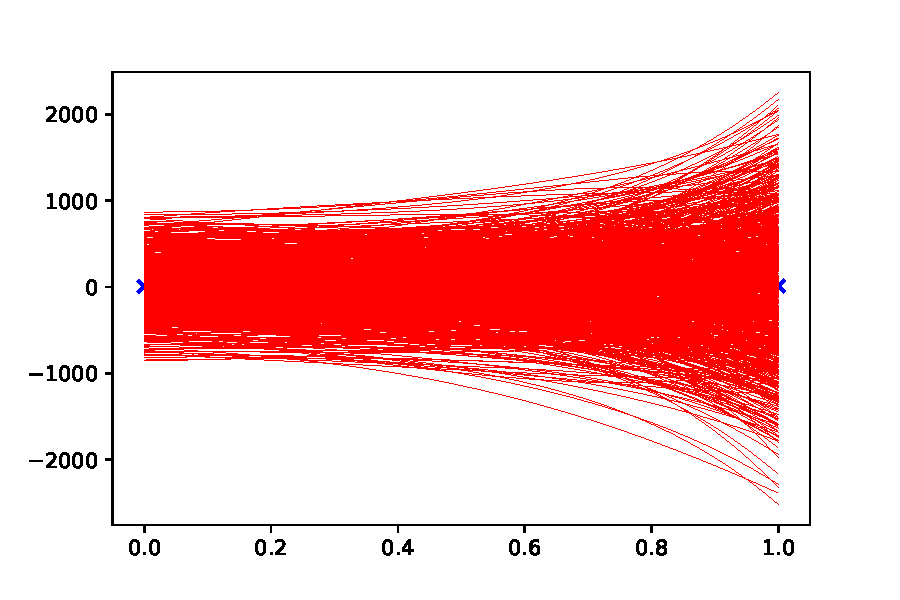
\includegraphics[width=\textwidth]{Q2_2.pdf}
         \caption{$\boldsymbol\omega \sim p(\boldsymbol\omega)$.}
     \end{subfigure}
     ~
     \begin{subfigure}[b]{0.45\textwidth}
         \centering
         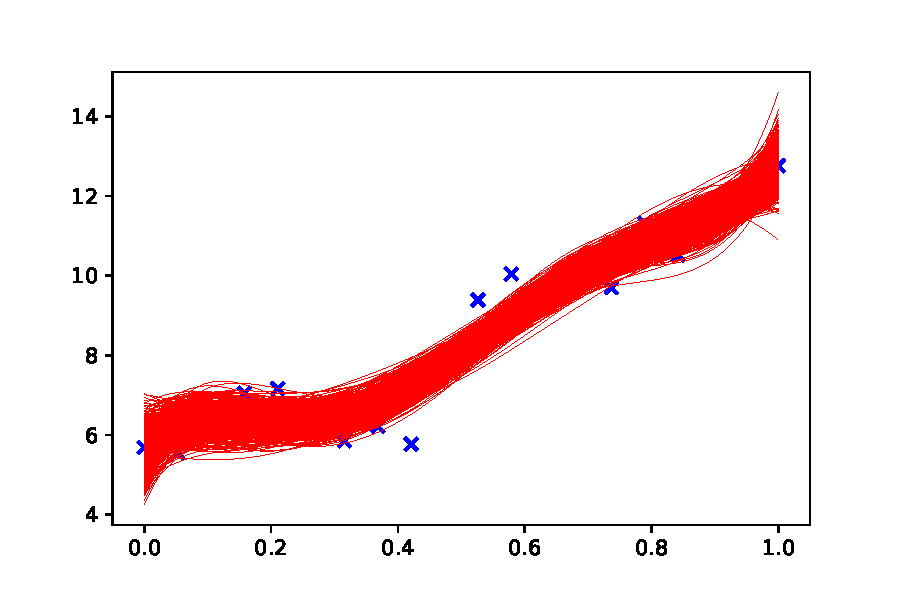
\includegraphics[width=\textwidth]{Q2_3.pdf}
         \caption{$\boldsymbol\omega \sim p(\boldsymbol\omega \vert \mathbf{y})$.}
     \end{subfigure}
     
     \caption{A visualisation of the samples from the prior and posterior distributions over $\boldsymbol\omega$.}
     \label{fig:Q2_sample_posterior}
\end{figure}

\subsubsection{The posterior predictive distribution}
The posterior distribution $p(\boldsymbol\omega \vert \mathbf{y})$ is only one half of the Bayesian inference process. We can use the posterior predictive distribution in Equation \eqref{eq:Q2_post_predict} to make predictions for new $x$ values. In Figure \ref{fig:Q2_post_predict} the posterior predictive distribution over the $x$ domain is shown.
\begin{figure}[htb!]
\centering
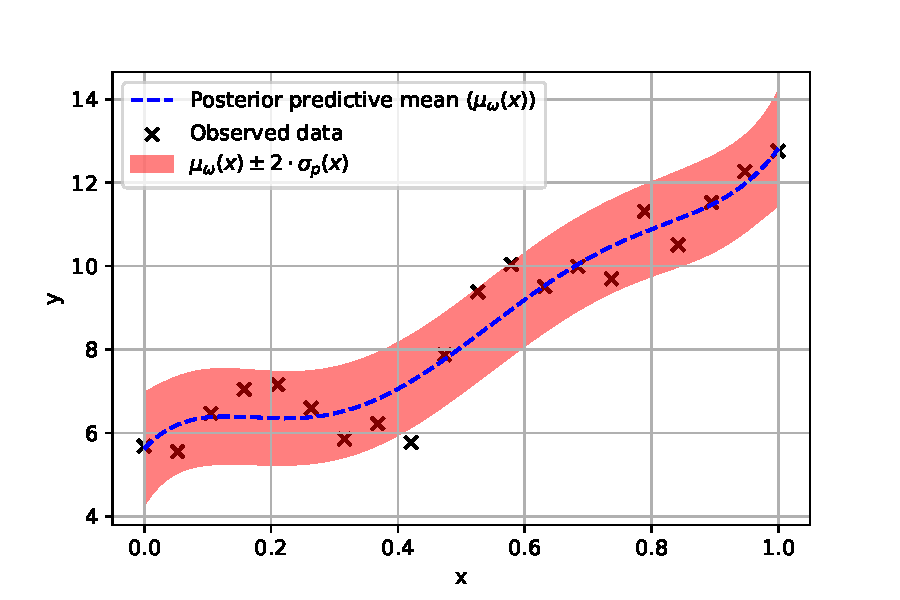
\includegraphics[scale=0.5]{Q2_4.pdf}
\caption{The posterior predictive distribution overlaid with the observed data.}
\label{fig:Q2_post_predict}
\end{figure}

\subsubsection{Bayesian inference interpretation}
Before we continue with the assignment, it is important that we reflect and comment on the distributions that we are using and the information they contain. The distributions discussed here are:
\begin{itemize}
\item The prior predictive distribution.
\item Functions generated from sampling the posterior distribution.
\item The posterior predictive distribution.
\end{itemize}

\textbf{The prior predictive distribution:} This distribution reflects our prior belief given to the generative model. The important aspect of this distribution is that it is a marginalisation over the model parameters for the product of the generative model and the prior distribution. As such, this distribution calculates the probability of a new data point $x$ given our prior uncertainty about the model parameters $\boldsymbol\omega$. The interpretation of this distribution is subjective, as it highly depends on our prior inference built into to the prior distribution. Hypothetically, if we expect that one regression parameter is not negative (such as the model offset $\omega_0$) then we could incorporate this prior knowledge into the prior distribution. This hypothetical process is subjective, as it depends on the user, and hence the prior predictive distribution will reflect this bias.

\textbf{Functions generated from sampling the posterior distribution:} Simply put, these functions represent different generative models. However, the posterior distribution represents the uncertainty in the parameter space given some observed data. As such, these functions represent are a proxy to the fit of the generative model to the observed data, where this fit has some uncertainty or variation (which is conveyed in the posterior distribution). If the functions vary greatly from sample to sample, then this is an indication that there is a large amount of uncertainty in the posterior distribution or the parameter space.

\textbf{The posterior predictive distribution:} The posterior predictive distribution is primarily used for predictive inference. This inference gives a distribution over an unobserved data point $x$, and it represents the process of integrating over an infinite number of models. Naturally, the posterior distribution conveys the uncertainty in the possible parameters for these different models, and hence gives an weighting to models that it believes are more likely given the observed data. This then allows the posterior predictive distribution to not only capture and express the uncertainty around a new data point, but it also serves as a proxy for us as to whether or not this new data is similar to the data that was previously observed.

\subsubsection{The impact of the prior hyper-parameters}
As before, the prior hyper-parameters influence the distributions obtained through the Bayesian inference process. The effects of $\alpha$ will be investigated. In this investigation, the model order will be linearly increased from 1 to 10. The objective is to investigate the effect of the model order on the ML estimate for $\boldsymbol\omega$, and the effect of the hyper-parameter $\alpha$ on the MAP estimate of $\boldsymbol\omega$ for different model orders. To quantify these effects, the mean-squared error (MSE) and the posterior-predictive log-likelihood will be inspected for different model orders and different values of $\alpha$. It is clear from Figure \ref{fig:Q2_hyper_parameters}a) that as the model order is increased, the generative model has more flexibility and thus appears more non-linear. In Figure \ref{fig:Q2_hyper_parameters}b) one can note that increasing $\alpha$ causes a gradual decrease in the posterior predictive log-likelihood. This gradual decrease, based on Figure \ref{fig:Q2_hyper_parameters}d), is attributed to the dominance of the prior in the Bayesian inference process. The prior enforces that the model parameters should be closer to zero, which acts as a form of regularisation on the model parameters. Hence, the expected values of the posterior predictive distribution for different model order become less non-linear as $\alpha$ increases. It is also clear to see that the posterior predictive log-likelihood steadies out after a model order of 2, which indicates that a second order polynomial fits that data well and additional model order do not have a significant impact. In Figure \ref{fig:Q2_hyper_parameters}c) an interesting response is observed, whereby as $\alpha$ is increased the MSE gets better up until $\alpha = 10$. From this point higher order models fit the data poorly in comparison to the lower-order variants.
\begin{figure}
\centering
\begin{subfigure}[b]{.45\textwidth}
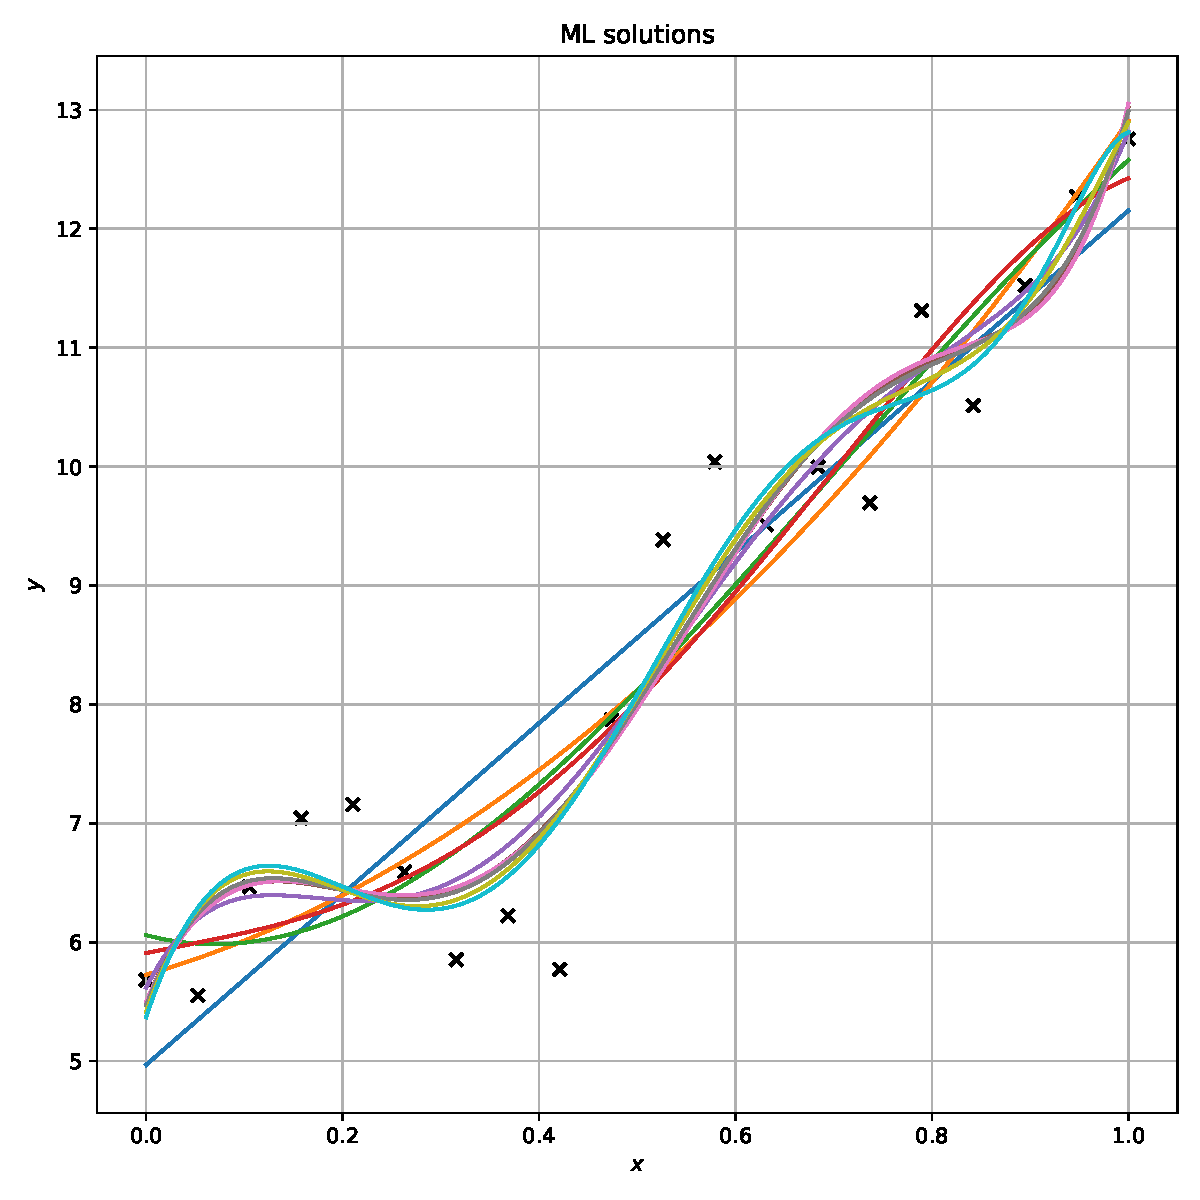
\includegraphics[width=\textwidth]{Q2_5.pdf}
\caption{ML estimates for $M = 1, \cdots, 10$.}

\vspace{2ex}

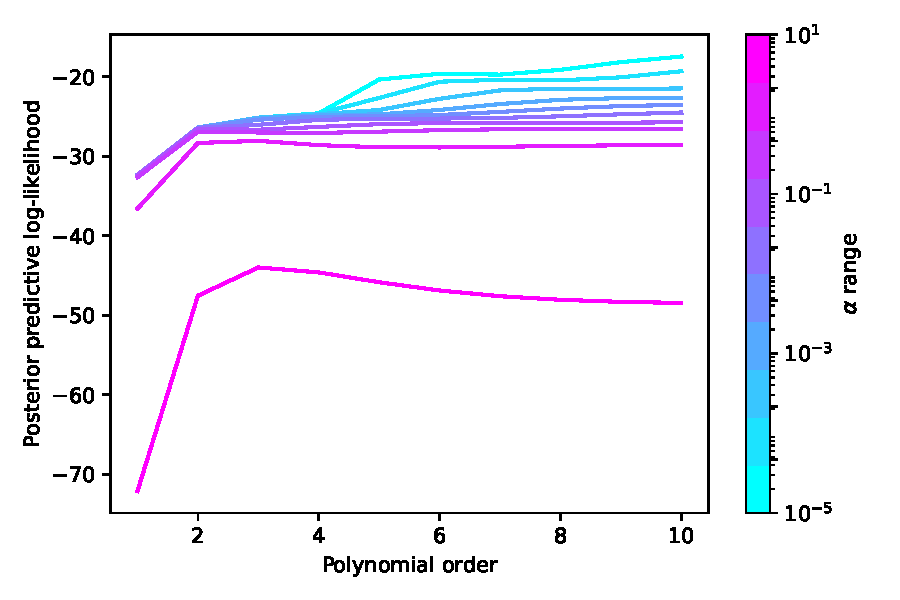
\includegraphics[width=\textwidth]{Q2_7.pdf}
\caption{Posterior predictive log-likelihood.}

\vspace{2ex}

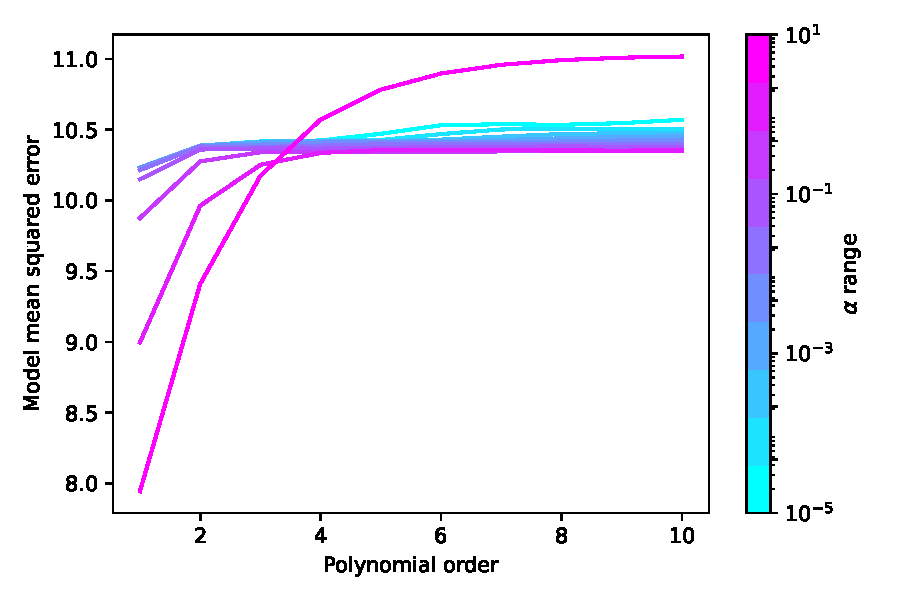
\includegraphics[width=\textwidth]{Q2_8.pdf}
\caption{Mean squared error.}

\end{subfigure}
\qquad
\begin{subfigure}[b]{.35\textwidth}
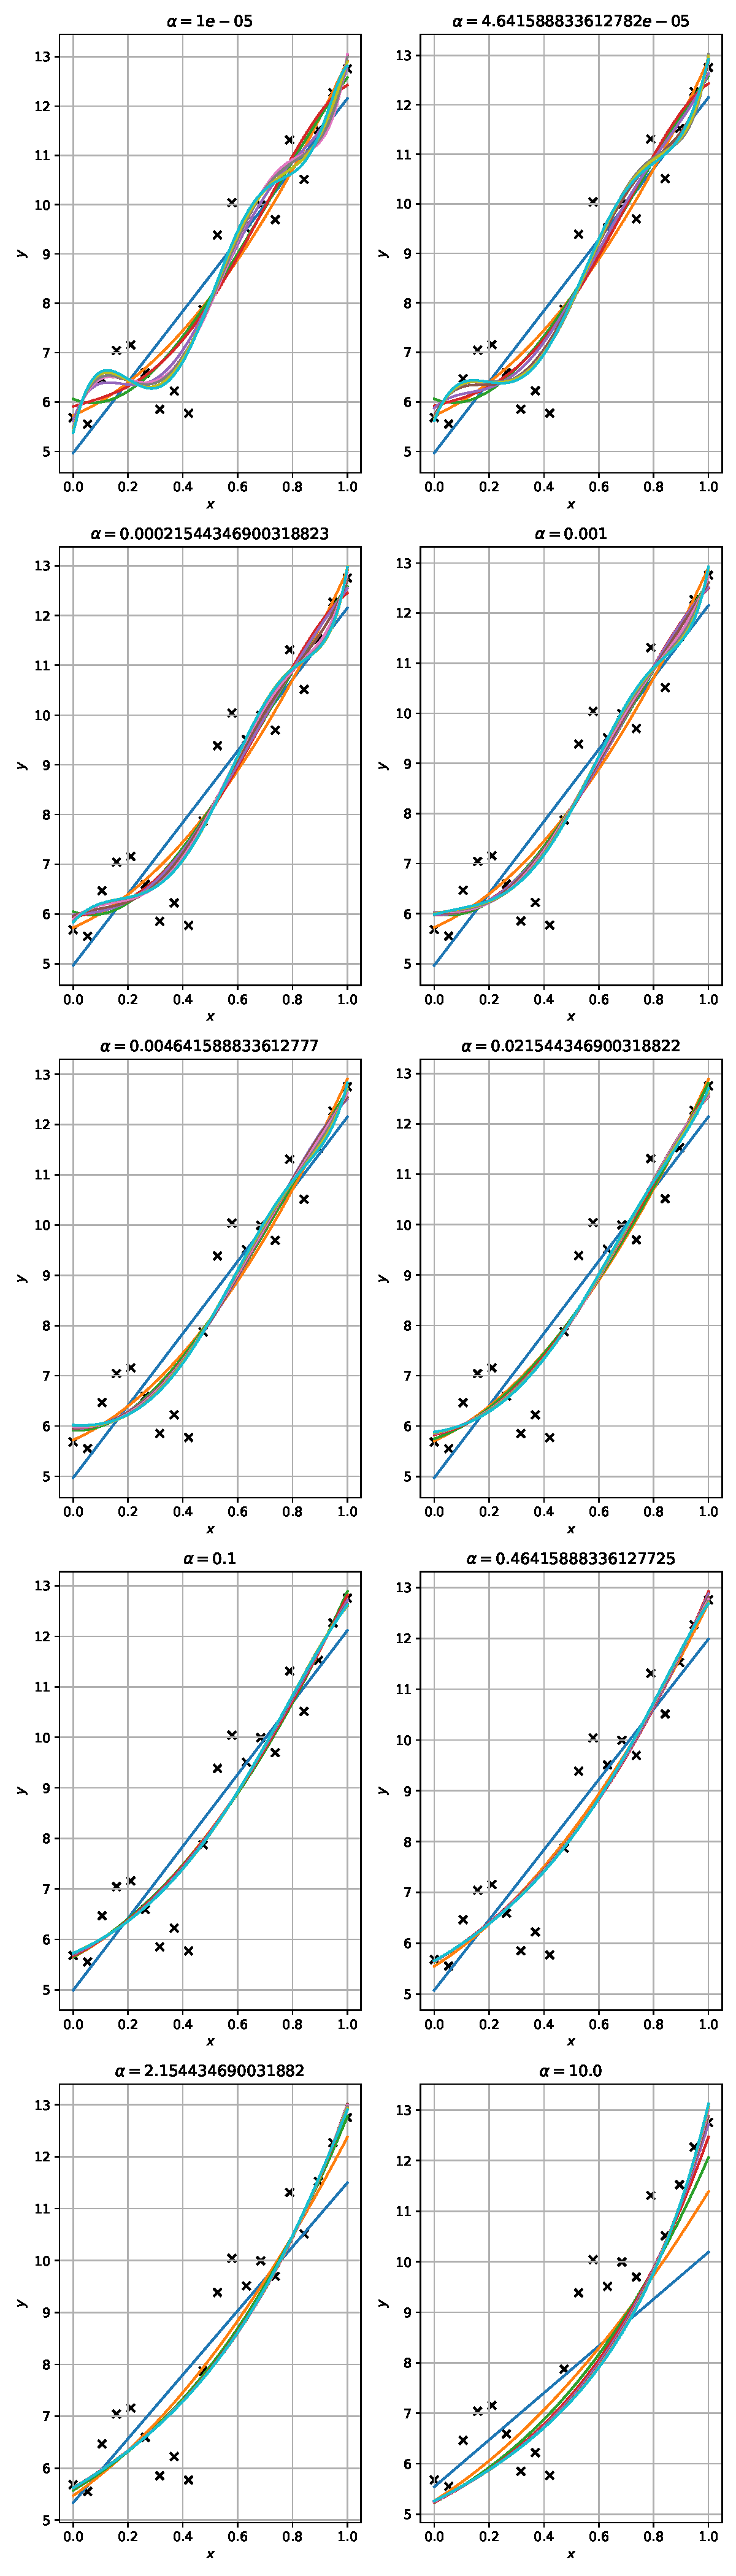
\includegraphics[width=\textwidth]{Q2_6.pdf}
\caption{Posterior predictive expected value visualisation.}
\end{subfigure}

\caption{The results of the $\alpha$ investigation. In a) the ML estimates for different model orders are shown, in b) the posterior-predictive log-likelihood for various $\alpha$ values and various model orders is shown, in c) the MSE for various $\alpha$ values and various model orders is shown, and in d) the expected values of the posterior predictive distribution are shown for the values of $\alpha$ considered in the investigation.}
\label{fig:Q2_hyper_parameters}
\end{figure}

\subsubsection{Interpreting the Bayesian inference results}
We can now use the prior distribution, posterior distribution, and posterior-predictive distribution to as questions regarding the model parameters and the predictive inference process. As the prior and posterior distributions are Gaussian, we can utilise the known properties of the Gaussian distribution to obtain the marginal distributions for the $\omega_1$ parameter. The details of this process are given in \citeauthor*{bishop2006} \cite{bishop2006}. As a result, the marginal distribution of interest for $P(\omega_1 > 8)$ is given by
\begin{equation}
p(\omega_1) = \mathcal{N}\left(\omega_1 \vert 0, \frac{1}{\alpha}\right).
\end{equation}
To calculate the probability $P(\omega_1 > 8 \vert \mathbf{x}, \mathbf{y})$, we can use the following Gaussian distribution
\begin{equation}
p(\omega_1 \vert \mathbf{x}, \mathbf{y}) = \mathcal{N}\left(\omega_1 \vert \mu_{\omega_1}, \Sigma_{\omega_{1,1}}) \right).
\end{equation}
Finally, to calculate the probability $P(y > 8 \vert x = 0.5, \mathbf{x}, \mathbf{y})$, we can use the posterior predictive distribution 
\begin{equation}
p(y \vert x = 0.5, \mathbf{x}, \mathbf{y}, \alpha, \beta) = \mathcal{N}(y \vert \boldsymbol\mu^{T}_{\boldsymbol\omega} \boldsymbol\phi(0.5), \sigma_p(0.5)^2)
\end{equation}

Note that our standard definition of probability is $P(x \leq a) = F_x(a)$. The probabilities of interest here, however, are $P(x > a)$ which can be expressed as
\begin{equation}
P(x > a) = 1 - P(x \leq a).
\end{equation}
The first probability $P(\omega_1 > 8)$ was found to be $P(\omega_1 > 8) = 1 - 0.5101 = 0.4899$. The second probability $P(\omega_1 > 8 \vert \mathbf{x}, \mathbf{y})$ of interest was found to be $P(\omega_1 > 8 \vert \mathbf{x}, \mathbf{y}) = 1 - 0.1561 = 0.8439$. The final probability of interest is $P(y > 8 \vert x = 0.5, \mathbf{x}, \mathbf{y})$ and this was determined to be $P(y > 8 \vert x = 0.5, \mathbf{x}, \mathbf{y}) = 1 - 0.4608 = 0.5392$. In Figure \ref{fig:Q2_CDFs} the CDFs of the prior, posterior and posterior-predictive distributions are shown. It is clear from Figure \ref{fig:Q2_CDFs}a) that the variance in the prior distribution is significant. This is expected as the ratio $\frac{1}{\alpha} = 10^5$. Thus, unless we evaluate the probability at the extremities of the prior, the probability will be close to 0.5. Hence the $\omega_1$ parameter can be sampled from an extensive range when using the prior. From Figure \ref{fig:Q2_CDFs}b), it is clear that the posterior distribution has a reduced variance. As such, the probability that the $\omega_1 > 8$ indicates that the parameter value is more likely to be larger than 8. Finally, as seen in Figure \ref{fig:Q2_CDFs}c), the posterior predictive distribution at $x = 0.5$ gives a distribution over $y$ that appears to be centred at 8. Hence, evaluating the probability that $y > 8$ returns a value close of 0.5, which indicates that a value of $y=8$ is highly likely at $x = 0.5$.
\begin{figure}[htb!]
     \centering
     \begin{subfigure}[b]{0.3\textwidth}
         \centering
         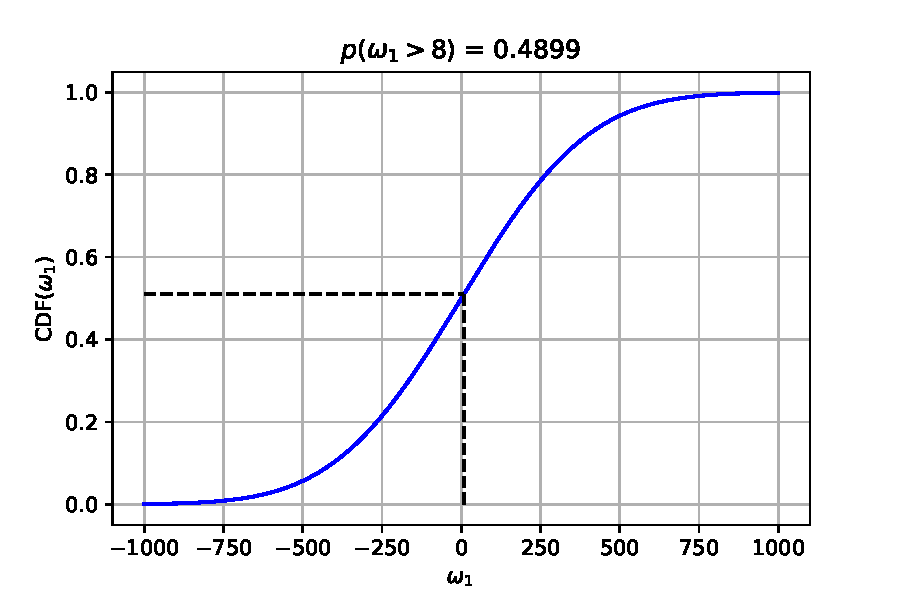
\includegraphics[width=\textwidth]{Q2_9.pdf}
         \caption{prior distribution.}
     \end{subfigure}
     ~
     \begin{subfigure}[b]{0.3\textwidth}
         \centering
         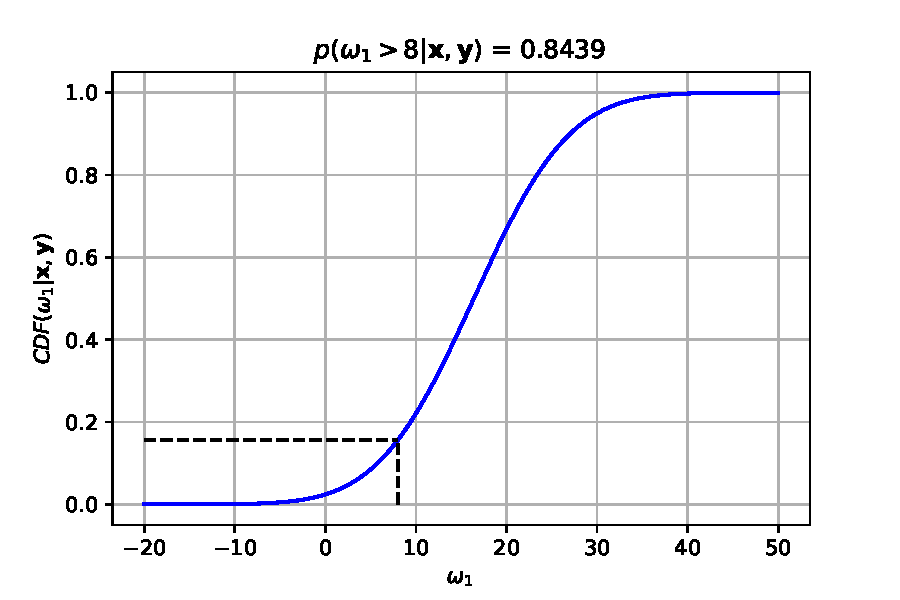
\includegraphics[width=\textwidth]{Q2_10.pdf}
         \caption{posterior distribution.}
     \end{subfigure}
     ~
     \begin{subfigure}[b]{0.3\textwidth}
         \centering
         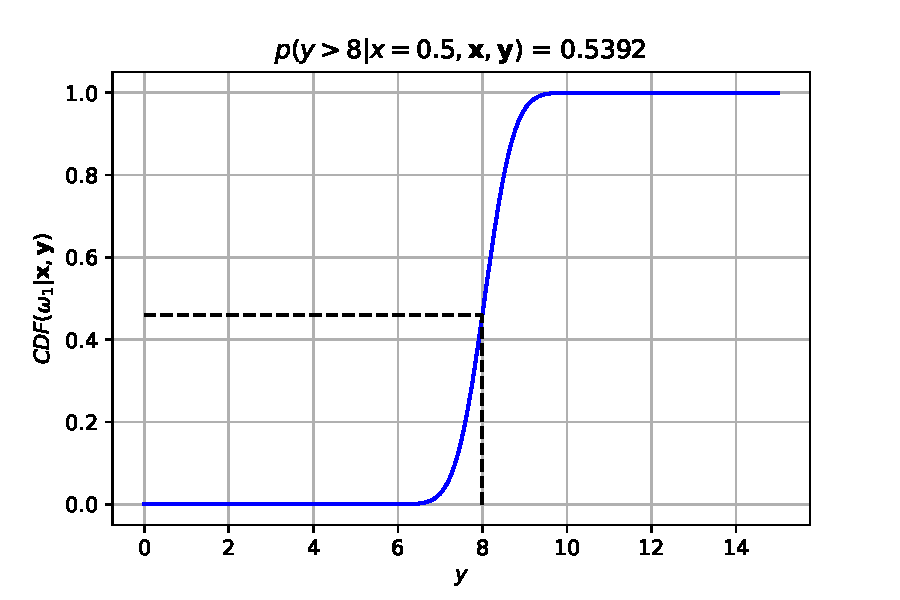
\includegraphics[width=\textwidth]{Q2_11.pdf}
         \caption{posterior-predictive distribution.}
     \end{subfigure}
     
     \caption{The CDFs of the prior, posterior, and posterior predictive distributions.}
     \label{fig:Q2_CDFs}
\end{figure}

\subsubsection{The model evidence}
In \citeauthor*{bishop2006} \cite{bishop2006}, the model evidence is given by
\begin{equation}
\ln p(\mathbf{y} \vert \alpha, \beta) = \frac{M}{2}\cdot \ln\alpha + \frac{N}{2}\cdot \ln \beta - E\left(\boldsymbol\mu_{\boldsymbol\omega}\right) - \frac{1}{2}\cdot \ln \vert \boldsymbol\Sigma^{-1}_{\boldsymbol\omega} \vert - \frac{N}{2}\cdot \ln (2 \cdot \pi),
\end{equation}
where $E\left(\boldsymbol\mu_{\boldsymbol\omega}\right)$ is given by
\begin{equation}
E\left(\boldsymbol\mu_{\boldsymbol\omega}\right) = \frac{\beta}{2} \Vert \mathbf{y} - \boldsymbol\Phi\boldsymbol\mu_{\boldsymbol\omega} \Vert_2^2 + \frac{\alpha}{2}\cdot \boldsymbol\mu_{\boldsymbol\omega}^T\boldsymbol\mu_{\boldsymbol\omega}.
\end{equation}

In Figure \ref{fig:Q2_evidence} the model evidence for different model orders and different values of the hyper-parameter $\alpha$ are shown. It is clear from Figure \ref{fig:Q2_evidence} that the parameter $\alpha$ has little to no sensitivity on the optimal model order until $\alpha = 0.1$. From this point, a higher model order is found to be desirable by the model evidence. This is attributed to the nature in which the  $\alpha$ hyper-parameter regularises the Bayesian inference process, and hence once this regularisation is strong, models with more flexibility are needed to overcome the effects of regularisation.
\begin{figure}[htb!]
     \centering
     \begin{subfigure}[b]{0.45\textwidth}
         \centering
         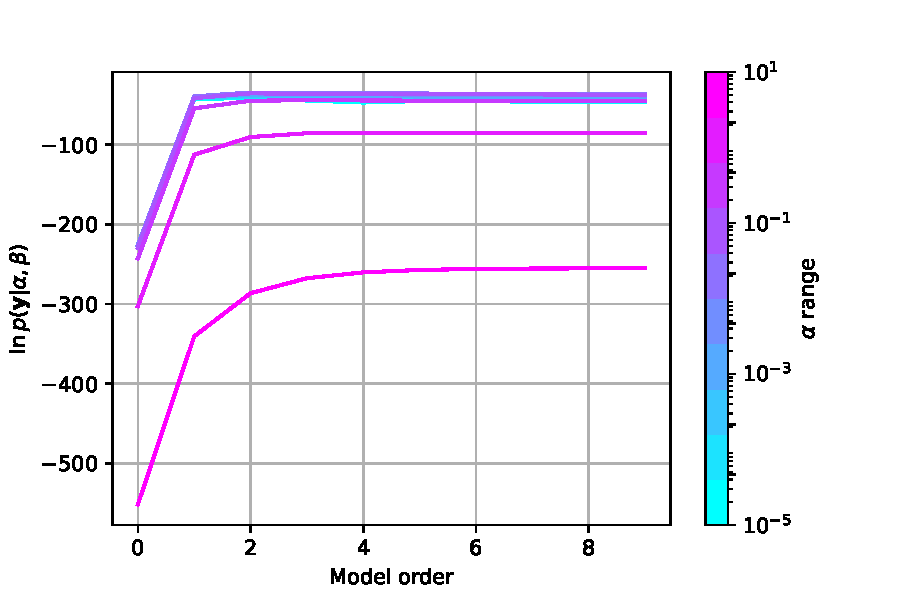
\includegraphics[width=\textwidth]{Q2_12.pdf}
         \caption{The model evidence.}
     \end{subfigure}
     ~
     \begin{subfigure}[b]{0.45\textwidth}
         \centering
         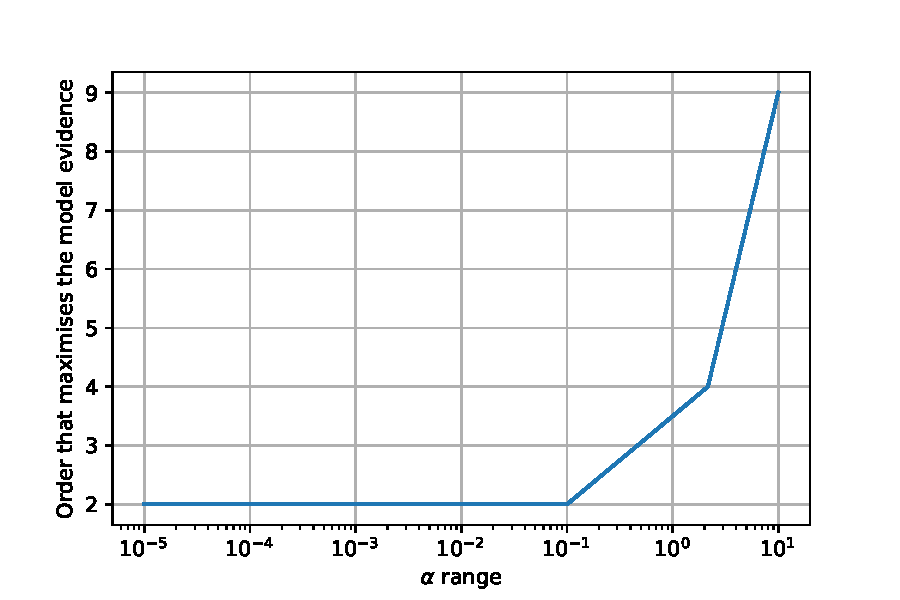
\includegraphics[width=\textwidth]{Q2_13.pdf}
         \caption{Optimal order versus $\alpha$.}
     \end{subfigure}
     
     \caption{The model evidence for different values of $\alpha$. In a) the model evidence is shown, and in b) the model order that maximises the model evidence for each value of $\alpha$ is plotted. }
     \label{fig:Q2_evidence}
\end{figure}

\subsubsection{Introducing sparsity}
Sparsity, in Bayesian inference, may be introduced to the model parameters through choices in the prior or through careful selection of the prior hyper-parameters. As was seen in this problem, if we increase $\alpha$ to a point where the prior variance is small, the resulting posterior predictive distribution and the MAP estimates of the model parameters is sparse. Alternatively, we could use a prior that is naturally sparse (i.e., it is strongly centered around zero) such as a Laplacian prior. The idea of sparsity is linked to regularisation, whereby the model parameters are constrained to ensure that the model does not overfit to the observed data. I would recommend looking into Laplacian priors or using the hyper-parameter $\alpha$ if one wishes to introduce sparsity into the Bayesian linear regression process.

Inducing sparsity differs from model evidence selection through the way that it interacts with the posterior distribution. A sparse prior, for example, has a direct influence on the posterior distribution, whereas the model evidence is the maximisation of the marginal likelihood function over the observed data for different model orders. While the posterior distribution does feature in this marginal likelihood, the prior has directly affects the methods used to determine the posterior distribution. 

\clearpage

\iffalse

\begin{figure}[htb!]
\centering
\includegraphics[scale=0.5]{.pdf}
\caption{words words words.}
\label{fig:}
\end{figure}

\begin{figure}[htb!]
     \centering
     \begin{subfigure}[b]{0.45\textwidth}
         \centering
         \includegraphics[width=\textwidth]{.pdf}
         \caption{sub-words.}
     \end{subfigure}
     ~
     \begin{subfigure}[b]{0.45\textwidth}
         \centering
         \includegraphics[width=\textwidth]{.pdf}
         \caption{sub-words.}
     \end{subfigure}
     
     \caption{words words words.}
     \label{fig:}
\end{figure}

\fi

\clearpage

%Print the bibliography
\printbibliography

\end{document}
